% format=twocolumn
\documentclass[]{report}
%\usepackage{mathptmx} % For svjour3 style font

\usepackage[a4paper, margin=1in]{geometry}

\usepackage[T1,T2A]{fontenc}
\usepackage[utf8]{inputenc}
\usepackage[english]{babel}
\usepackage{amsmath,amssymb}
\usepackage{mathtext}
\usepackage{amsthm}
\usepackage{graphicx}
\usepackage{cmap}
\usepackage{bbm}
\usepackage{tikz}
\usepackage{float}

\usepackage[backend=biber,style=alphabetic,sorting=ynt]{biblatex}
\usepackage{csquotes}
\addbibresource{bibliography.bib}

\usepackage{graphicx}

% Types

\newtheorem{theorem}{Theorem}
\newtheorem{lemma}{Lemma}
\newtheorem{proposition}{Proposition}
\newtheorem{col}{Corrolary}

\theoremstyle{definition}
\newtheorem{definition}{Definition}

\theoremstyle{definition}
\newtheorem{example}{Example}

\theoremstyle{definition}
\newtheorem*{nb}{NB}


\newcommand{\hm}[1]{#1\nobreak\discretionary{}{\hbox{\ensuremath{#1}}}{}}

\DeclareMathOperator{\sgn}{sign}
\DeclareMathOperator*{\var}{var}   
\DeclareMathOperator*{\cov}{cov}

\newcommand{\1}{\mathbbm{1}} 
\newcommand{\R}{\mathbb{R}}
\newcommand{\N}{\mathbb{N}}
\renewcommand{\P}{P}
\newcommand{\eps}{\varepsilon}

\newcommand\cA{{\cal A}}
\newcommand\cE{{\cal E}}
\newcommand\cC{{\cal C}}
\newcommand\cF{{\cal F}}
\newcommand\cG{{\cal G}}
\newcommand\cK{{\cal K}}
\newcommand\cL{{\cal L}}
\newcommand\cB{{\cal B}}
\newcommand\cN{{\cal N}}
\newcommand\cM{{\cal M}}
\newcommand\cX{{\cal X}}
\newcommand\cD{{\cal D}}
\newcommand\cR{{\cal R}}
\newcommand\cP{{\cal P}}
\newcommand\cQ{{\cal Q}}
\newcommand\cS{{\cal S}}
\newcommand\cT{{\cal T}}
\newcommand\cV{{\cal V}}
\newcommand\cZ{{\cal Z}}

\newcommand{\wt}{\widetilde}

\numberwithin{equation}{section}
\numberwithin{theorem}{section}
\numberwithin{lemma}{section}
\numberwithin{proposition}{section}
\numberwithin{col}{section}
\numberwithin{definition}{section}
\numberwithin{example}{section}

\usepackage{hyperref}
\hypersetup{
	colorlinks=true,
	linkcolor=blue,
	filecolor=magenta,      
	urlcolor=cyan,
	citecolor=black
}

\title{'Pricing under Rough Volatilty Models' Lab Report \\ \ \\ Group 2}
\author{Artemy Sazonov \and Andrei Petrov \and Maxim Savostyanov}

\begin{document}
    \maketitlepage

    \pagenumbering{roman}

    \begin{abstract}
        In the present paper we investigate the roughness of the Russian stock market. 
In order to do this, we study the behavior of the Zumbach effect in real market data and 
non-rough stochastic volatility model Monte-Carlo simulations. After that we study the RFSV 
model and we obtain the estimation of the Hurst parameter for the 
major Russian corporations. Futhermore, we investigate the sample normalized variation statistic 
and see that roughness could vary depending on estimation of volatility.
    \end{abstract}

    \addcontentsline{toc}{chapter}{Table of Contents}\tableofcontents

    \addcontentsline{toc}{chapter}{List of Figures}\listoffigures
    \addcontentsline{toc}{chapter}{List of Tables}\listoftables

    
    \chapter*{Introduction}\pagenumbering{arabic}\setcounter{page}{3}\addcontentsline{toc}{chapter}{Introduction}

        \section{Introduction}

    \chapter{Basic Theoretical Aspects}

        \section{Realized volatility}
    Consider a stochastic volatility model 
    \begin{equation}\label{model:SVM}
        dS_t = \mu_t S_t dt + \sigma_t S_tdW_t,
    \end{equation}
    where $S_t$ is an asset price process, and $\sigma_t$ is a stochastic volatility process representing a so-called \emph{spot volatility}.
    Spot volatility, in fact, is not observable in the market, therefore, we should estimate it somehow.

    \begin{definition}
        The \emph{realized variance} of a price process $S$ over time interval $[t, t + \delta]$ sampled along the time partition $\pi^n$
        is defined as 
        \begin{equation}\label{def:RV}
            RVar_{t, t + \delta}(\pi^n) = \sum_{\pi^n \cap [t, t + \delta]} \left(\log S_{t^n_{i+1}} - \log S_{t^n_{i}}\right)^2
        \end{equation}
        and \emph{realized volatility} is defined as
        \begin{equation}\label{def:RVol}
            RV_{t, t + \delta}(\pi^n) = \sqrt{\sum_{\pi^n \cap [t, t + \delta]} \left(\log S_{t^n_{i+1}} - \log S_{t^n_{i}}\right)^2}
        \end{equation}
    \end{definition}

    \begin{definition}
        Let $S$ satisfy \eqref{model:SVM}. Then the integrated variance is defined as
        \begin{equation}\label{def:IV}
            IVar_t = \int_{0}^{t} \sigma_s^2 ds
        \end{equation}
    \end{definition}
    It has been shown many times (e.g. \cite{Barndorff-Nielsen2002}) and mentioned in \cite{Cont2022} that the realized variance converges 
    in probability to the integrated variance as sampling frequency increases for all assets satistying the equation 
    \eqref{model:RFSVasset} (i.e. stochastic volatility models).
    \begin{proposition} 
        As time partition scale of $\pi^n$ tends to $0$, $RV_{t, t + \delta}(\pi^n) \approx \sqrt{\delta} \sigma_t$, i.e. $RV_{t, t + \delta}/\sqrt{\delta}$ could be considered as a consistent estimator of the spot volatility.
    \end{proposition}

    \begin{definition}
        The \emph{fractional Brownian motion} $(W_t^H)_{t\in \mathbb{R_+}}$ with Hurst 
        parameter $H \in (0, 1)$ is a Gaussian process with the following properties:
        \begin{enumerate}
            \item $W_0^H = 0$,
            \item $\mathbb{E}\left[W_t^H\right] \equiv 0$,
            \item $\mathbb{E}\left[W_s^H W_t^H\right] = \frac{1}{2} \left(t^{2H} + s^{2H} - |t-s|^{2H}\right)$
        \end{enumerate}
    \end{definition}

    \begin{definition}
        A stationary fOU process $X_t$ is defined as the stationary solution of the stochastic differential equation
        \begin{equation}
            dX_t = \nu dW^H_t - \alpha (X_t - m)dt,
        \end{equation}
        where $m \in \mathbb{R}$ and $\nu$ and $\alpha$ are positive parameters, see \cite{Cheridito2003}.
    \end{definition}

    \subsection{What is a long-memory process?}
        \begin{definition}
            A process $X_t$ is said to have a long memory, if 
            \begin{equation}
                \sum_{k=0}^{\infty}Cov\left[X_1 , X_{k} - X_{k-1}\right] = +\infty.
            \end{equation}
        \end{definition}

        In particular, the fractional Brownian motion with $H > \frac{1}{2}$ is a long-memory process.
        Long-memory of the stochastic volatility process in stochastic volatilty models framework used to be a 
        widely-accepted stylized fact \cite{Breidt1998,ComteRenault1998,Comte1996,Ding1993}.

        \section{Normality Statistical Tests}\label{sec:statisticaltest}
        In the following, $x_i$ denotes a sample of $n$ observations, $g_1$ and $g_2$ are the sample 
        skewness and kurtosis, $\mu_j$'s are the $j$-th sample central moments, and $\overline{x}$ is the 
        sample mean. 
        \subsection{D'Agostino's K-squared test}
            The sample skewness and kurtosis are defined as
            \begin{align}
                & g_1 = \frac{ m_3 }{ m_2^{3/2} } = \frac{\frac{1}{n} \sum_{i=1}^n \left( x_i - \overline{x} \right)^3}{\left( \frac{1}{n} \sum_{i=1}^n \left( x_i - \overline{x} \right)^2 \right)^{3/2}}\ , \\
                & g_2 = \frac{ m_4 }{ m_2^{2} }-3 = \frac{\frac{1}{n} \sum_{i=1}^n \left( x_i - \overline{x} \right)^4}{\left( \frac{1}{n} \sum_{i=1}^n \left( x_i - \overline{x} \right)^2 \right)^2} - 3\ .
            \end{align}
            Let
            \begin{equation}
                Z_1(g_1) = \delta \operatorname{asinh}\left( \frac{g_1}{\alpha\sqrt{\mu_2}} \right),
            \end{equation}
            where constants $\alpha$ and $\delta$ are computed as
            \begin{align}
                & W^2 = \sqrt{2\gamma_2 + 4} - 1, \\
                & \delta = 1 / \sqrt{\ln W}, \\
                & \alpha^2 = 2 / (W^2-1),
            \end{align}
            and
            \begin{equation}
                Z_2(g_2) = \sqrt{\frac{9A}{2}} \left\{1 - \frac{2}{9A} - \left(\frac{ 1-2/A }{ 1+\frac{g_2-\mu_1}{\sqrt{\mu_2}}\sqrt{2/(A-4)} }\right)^{\!1/3}\right\},  
            \end{equation}
            where
            \begin{align}
                & A = 6 + \frac{8}{\gamma_1} \left( \frac{2}{\gamma_1} + \sqrt{1+4/\gamma_1^2}\right), \\
                & \mu_1(g_2) = - \frac{6}{n+1}, \\
                & \mu_2(g_2) = \frac{ 24n(n-2)(n-3) }{ (n+1)^2(n+3)(n+5) }, \\
                & \gamma_1(g_2) \equiv \frac{\mu_3(g_2)}{\mu_2(g_2)^{3/2}} = \frac{6(n^2-5n+2)}{(n+7)(n+9)} \sqrt{\frac{6(n+3)(n+5)}{n(n-2)(n-3)}},  \label{eq:gamma1}\\
                & \gamma_2(g_2) \equiv \frac{\mu_4(g_2)}{\mu_2(g_2)^{2}}-3 = \frac{ 36(15n^6-36n^5-628n^4+982n^3+5777n^2-6402n+900) }{ n(n-3)(n-2)(n+7)(n+9)(n+11)(n+13) }\label{eq:gamma2}.
            \end{align}
            The analytical expressions for skewness and kurtosis \eqref{eq:gamma1} - \eqref{eq:gamma2} were derived by E. Pearson in \cite{Pearson1931}.
            \begin{definition}
                The \emph{D'Agostino-Pearson} statistic is defined as 
                \begin{equation}
                    K^2 = Z_1(g_1)^2 + Z_2(g_2)^2
                \end{equation}
                Null hypothesis: the sample is normally distributed.
            \end{definition}
    
            \begin{nb}
                The $K^2$ statistic is able to detect deviations from both skewness and kurtosis. 
                If the null hypothesis is true, then the test statistic has the $\chi^2$ 
                distribution with $2$ degrees of freedom. 
            \end{nb}
    
        \subsection{Shapiro-Wilk test}
            \begin{definition}
                The Shapiro–Wilk test statistic is defined as
                \begin{equation}
                    W = \frac{\left(\sum_{i=1}^n a_i x_{(i)}\right)^2}{\sum_{i=1}^n (x_i-\overline{x})^2},
                \end{equation}
                where
                \begin{equation*}
                    (a_1, \dots, a_n) = \frac{m^{T} V^{-1}}{C}, \quad C = \| V^{-1} m \| = (m^{T} V^{-1}V^{-1}m)^{1/2},
                \end{equation*}
                and $m = (m_1, \dots, m_n)^{T}$ is a mean of order statistic from a normally distributed sample, $V$ is the covariance matrix of those normal order statistics. 
                Null hypothesis: the sample is normally distributed.
            \end{definition}
    
            \begin{nb}
                The $W$ statistic has no distinguishable name, and the cutoff values are calculated numerically by Monte-Carlo simulation.
            \end{nb}

    \chapter{Zumbach Effect Estimation}

        \section{Empirical Effect}
    

        \section{Monte-Carlo Simulation of Zumbach Effect}
    

        We conclude that Zumbach effect is an argument for the roughness of volatility. Therefore, we should consider a model of volatility driven by fractional Brownian motion.

    \chapter{Rough Fractional Stochastic Volatilty Model Estimation}

        

\section{Model description}
    In \cite{GatheralRosenbaum2014} the authors considered the following model. 
    Let there be a riskless asset $B_t \equiv 1$, and a risky asset, whose price $S_t$ is defined 
    by the following equations: 
    \begin{align}
        & dS_t          = \alpha S_t dt + \sigma_t S_tdW_t,               \label{model:RFSVasset} \\
        & d\log\sigma_t = \alpha (m - \log\sigma_t) dt + \nu dW_t^H.      \label{model:RFSVvol}
    \end{align}
    The risky asset is being traded in the market in numeraire prices. In our case, $B_t = 1$ RUB for stocks and $1$ GBP for depositary reciepts.
    \begin{definition}
        A model \eqref{model:RFSVasset} -- \eqref{model:RFSVvol} is called a 
        \emph{Fractional Stochastic Volatility Model} (FSV). For a special case $H < 0.5$ the 
        model is called a \emph{Rough Fractional Stochastic Volatility Model} (RFSV) to emphasise a 
        so-called roughness of the trajectories of the fBm. 
        As a stylized fact we shall demand the stationarity of log-increments.
    \end{definition}

    In \cite{Cheridito2003} an exact formula for the autocovariance function of the log-volatility in the RFSV model was derived:
    \begin{multline}\label{formula:CovLog}
        \cov\left[\log \sigma_{t}, \log \sigma_{t+\Delta}\right] =\\= \frac{H(2H-1)\nu^2}{2\alpha^{2H}}\left(e^{-\alpha\Delta} \Gamma(2H-1) + e^{-\alpha\Delta} \int_{0}^{\alpha\Delta}\frac{e^u}{u^{2-2H}}du + e^{\alpha\Delta} \int_{\alpha\Delta}^{\infty}\frac{e^u}{u^{2-2H}}du\right).
    \end{multline}
    Let $m(q, \Delta, \pi^n)$ be a sample $q$-th absolute moment of $\log RV_{t+\Delta} - \log RV_t$:
    \begin{equation}
        m(q, \Delta, \pi^n) := \frac{1}{n} \sum_{t} \left|\log RV_{t + \Delta} - \log RV_t\right|^q,
    \end{equation}
    i.e. $m(q, \Delta, \pi^n)$ is an empirical counterpart of $\mathbb{E}\left[\left|\log RV_{\Delta} - \log RV_0\right|^q\right]$.
    In this work we shall use the uniform partition of time scale with each step being equal to $15$ minutes, so we omit the $\pi^n$ notation and use $m(q, \Delta)$.
    Via the explicit formula for the covariance function of the log-volatility in the RFSV model \eqref{formula:CovLog}, we can write 
    a closed-form expression for a theoretical $m(2, \Delta)$:
    \begin{equation}
        m(2, \Delta) = 2\left(\var \log\sigma_{t} - \cov\left[\log\sigma_{t}, \log\sigma_{t+\Delta}\right]\right).
    \end{equation}


        \section{Statistical Analysis}
    \subsection{Data Preprocessing and Realized Volatility Estimation}
        In the present paper we used high-frequency data for three types of assets:
        \begin{enumerate}
            \item\textbf{Stocks}: Yandex, Sberbank, Gazprom, VTB, Moscow Exchange, Lukoil, and X5 Group
            \item\textbf{Depositary reciepts}: Sberbank, Gazprom, VTB, and Lukoil
            \item\textbf{Funds}:
        \end{enumerate}

        \begin{figure}[htbp]
            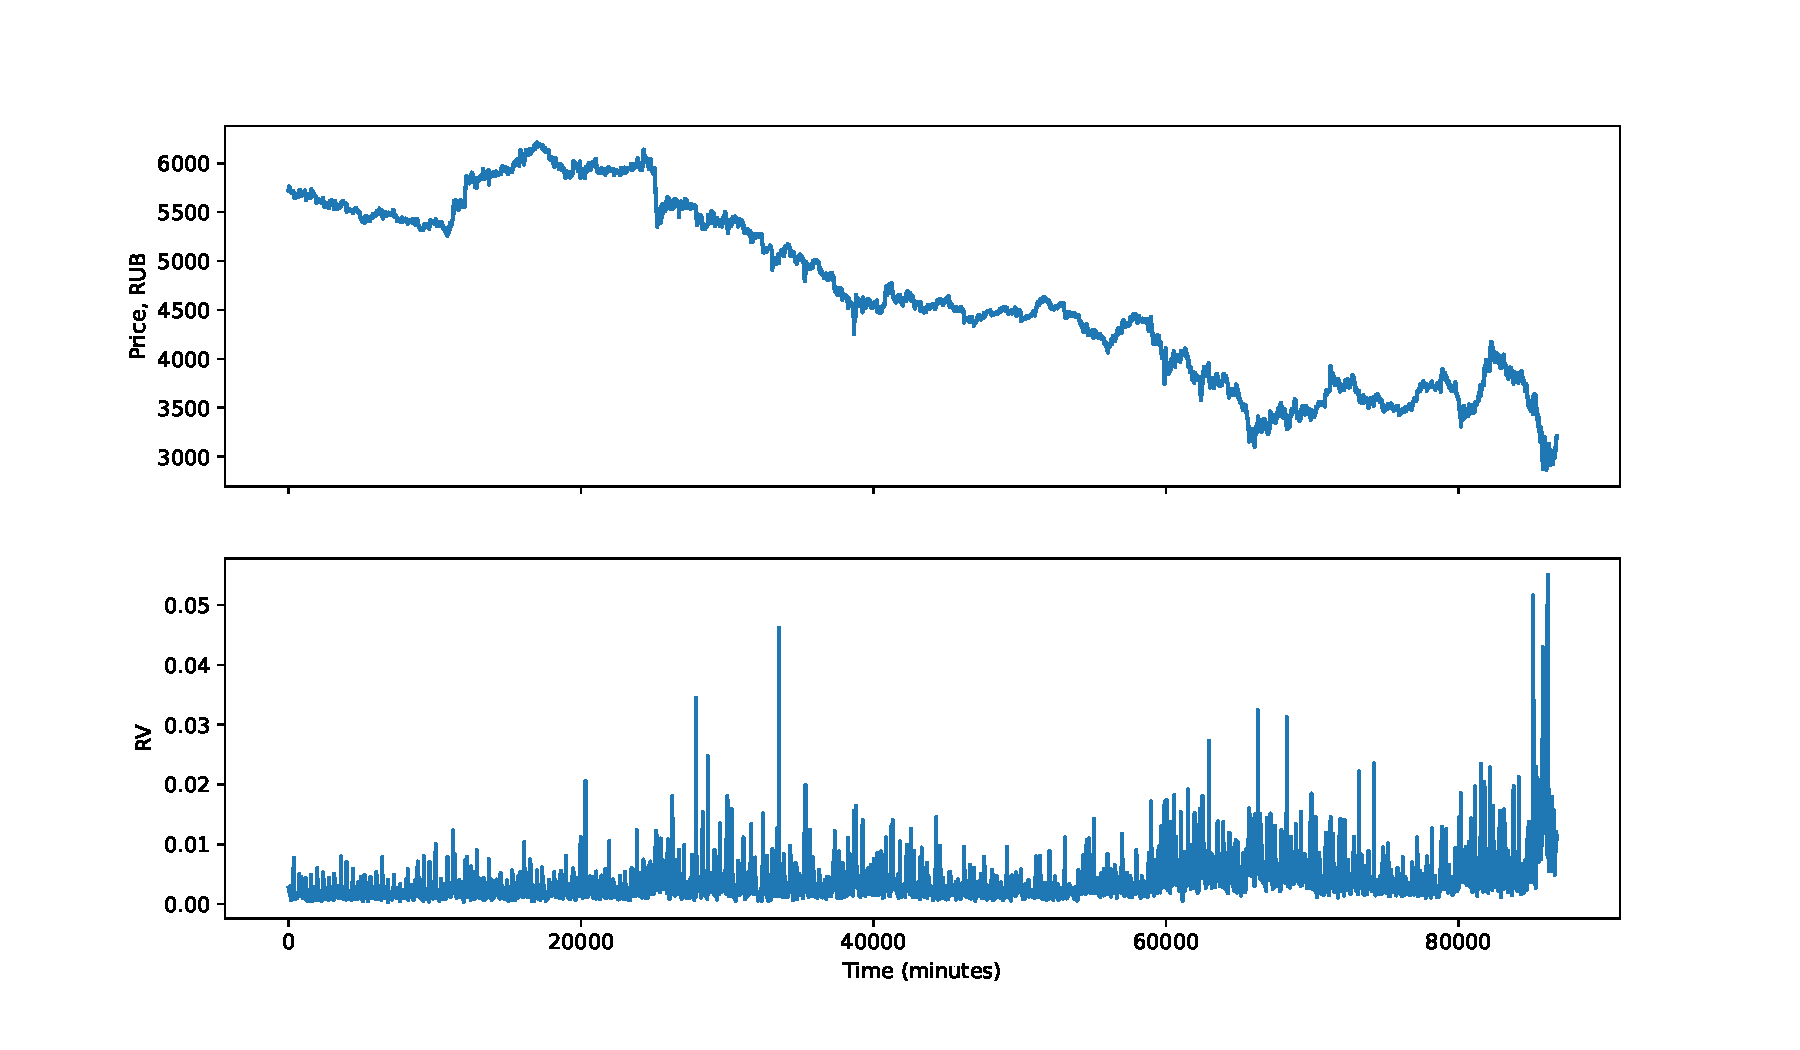
\includegraphics[width=\textwidth]{fig/YNDX RX Equity RVol.pdf}
            \caption{YNDX RX Equity. Price and Realized Volatility}
        \end{figure}

        Some text to be written

        Using this approach to estimate the realized volatility we can be sure that our data is correlated in the least way possible.

    \subsection{Hurst Parameter Estimation}
        Let $m(q, \Delta, \pi^n)$ be a sample $q$-th absolute moment of $\log RV_{t+\Delta} - \log RV_t$ 
        (under stationarity of increments assumptions):
        \begin{equation}
            m(q, \Delta, \pi^n) := \frac{1}{n} \sum_{t} \left|\log RV_{t + \Delta} - \log RV_t\right|^q,
        \end{equation}
        i.e. $m(q, \Delta, \pi^n)$ is an empirical counterpart of $\mathbb{E}\left[\left|\log RV_{\Delta} - \log RV_0\right|^q\right]$. 
        In my work we used the uniform partition with $\Delta$-minutes increments, so we omit the $\pi^n$ notation and use $m(q, \Delta)$.

        Due to the similarities in the obtained results for all assets, we shall deeply analyze the Hurst parameter estimation only for the 
        Yandex stocks (YNDX RX Equity). Plots for other equities could be found in the appendix, whereas the Hurst parameter estimations for them 
        could be found in the table \ref{table:hurst_est}. 
        Estimation parameters:
        \begin{itemize}
            \item Realized volatility is estimated by 15 minute disjoint windows
            \item $\Delta \in [0, 40]$ for $\zeta_q$ estimation and other plots
        \end{itemize}

        \begin{nb}
            We did not manage to obtain more HF data (only 5 months of 1m-tick data), therefore my estimations are not precise and could 
            not be used for further application.
        \end{nb}

        \begin{table}[htbp]
            \centering
            \begin{tabular}{|c|c|c|}
                \hline
                Asset Type               & Ticker & $\hat H$  \\ \hline
                \hline
                Stock                    & YNDX   & 0.0521766 \\ \hline
                Stock                    & SBER   & 0.1551646 \\ \hline
                Stock                    & VTBR   & 0.0917236 \\ \hline
                Stock                    & MOEX   & 0.0853878 \\ \hline
                Stock                    & LKOH   & 0.0730521 \\ \hline
                Stock                    & GAZP   & 0.1309705 \\ \hline
                Stock                    & FIVE   & 0.0630289 \\ \hline
                \hline
                Depositary reciept       & OGZD   & 0.0523981 \\ \hline
                Depositary reciept       & VTBR   & 0.0370185 \\ \hline
                Depositary reciept       & SBER   & 0.0578053 \\ \hline
                Depositary reciept       & LKOD   & 0.0352792 \\ \hline
                \hline
                Index                    & .AEX & 0.1271101 \\ \hline
                Index                    & .AORD & 0.0731749 \\ \hline
                Index                    & .BFX & 0.1340391 \\ \hline
                Index                    & .BVSP & 0.1285106 \\ \hline
                Index                    & .DJI & 0.1176993 \\ \hline
                Index                    & .FCHI & 0.1300797 \\ \hline
                Index                    & .FTMIB & 0.139092 \\ \hline
                Index                    & .FTSE & 0.0958701 \\ \hline
                Index                    & .GDAXI & 0.1130176 \\ \hline
                Index                    & .GSPTSE & 0.0910194 \\ \hline
                Index                    & .HSI & 0.0893922 \\ \hline
                Index                    & .IBEX & 0.1028588 \\ \hline
                Index                    & .IXIC & 0.1278909 \\ \hline
                Index                    & .KS11 & 0.1066547 \\ \hline
                Index                    & .KSE & 0.1080452 \\ \hline
                Index                    & .MXX & 0.0673153 \\ \hline
                Index                    & .N225 & 0.1063503 \\ \hline
                Index                    & .OMXC20 & 0.0997755 \\ \hline
                Index                    & .OMXHPI & 0.0954135 \\ \hline
                Index                    & .OMXSPI & 0.118664 \\ \hline
                Index                    & .OSEAX & 0.0987837 \\ \hline
                Index                    & .RUT & 0.1029421 \\ \hline
                Index                    & .SMSI & 0.1319457 \\ \hline
                Index                    & .SPX & 0.1328797 \\ \hline
                Index                    & .SSEC & 0.1170868 \\ \hline
                Index                    & .SSMI & 0.1469914 \\ \hline
            \end{tabular}
            \caption{Hurst parameter estimations}
            \label{table:hurst_est}
        \end{table}



        In the figure \ref{fig:logMDelta} we can see that for $q = 0.6, 0.8, \text{and} 1.0$ the dots are very discrepant for $\log\Delta > 2.0$. 
        However, we get a pretty decent linear fit for $q = 0.2$ and $q = 0.4$, therefore, the estimation on these two point would be the best one
        we can manage to extract. On the other hand, on $\zeta_q$ plot we observe a perfect linear fit for all $q$-s, therefore, $H$
        is its slope indeed.

        \begin{figure}[htbp]
            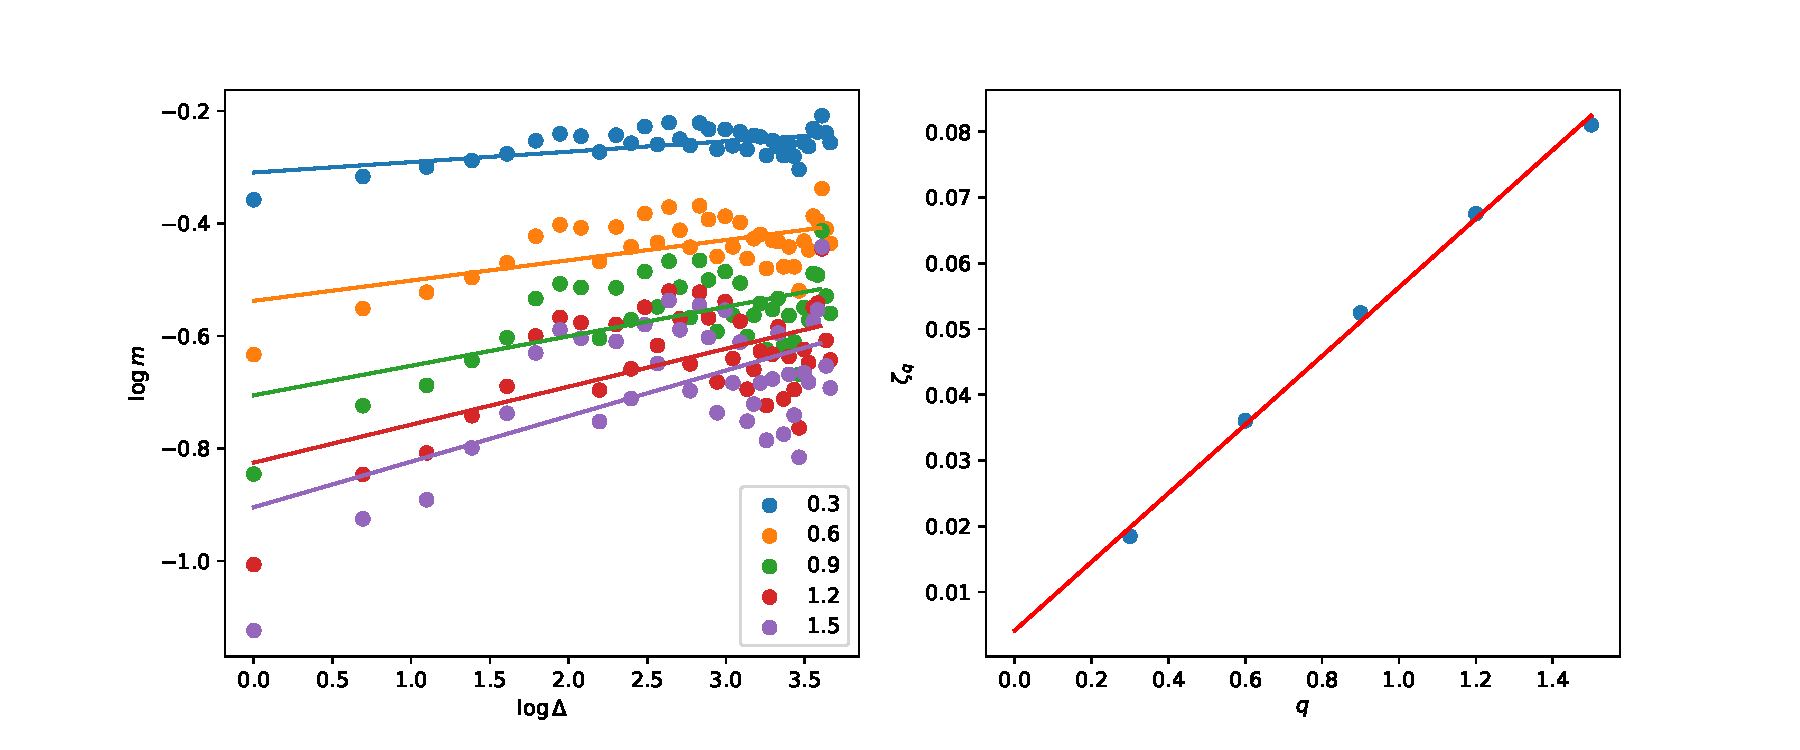
\includegraphics[width=\textwidth]{fig/YNDX RX Equity Hurst Est.pdf}
            \caption{YNDX RX Equity. Plots for $\hat{H}$}
            \label{fig:logMDelta}
        \end{figure}

        We note that the graphs for $\zeta_q$ are slightly concave, which correlates with \cite{GatheralRosenbaum2014} results.
        They conclude that this effect takes place due to the finite statistical population size.

        \begin{figure}
            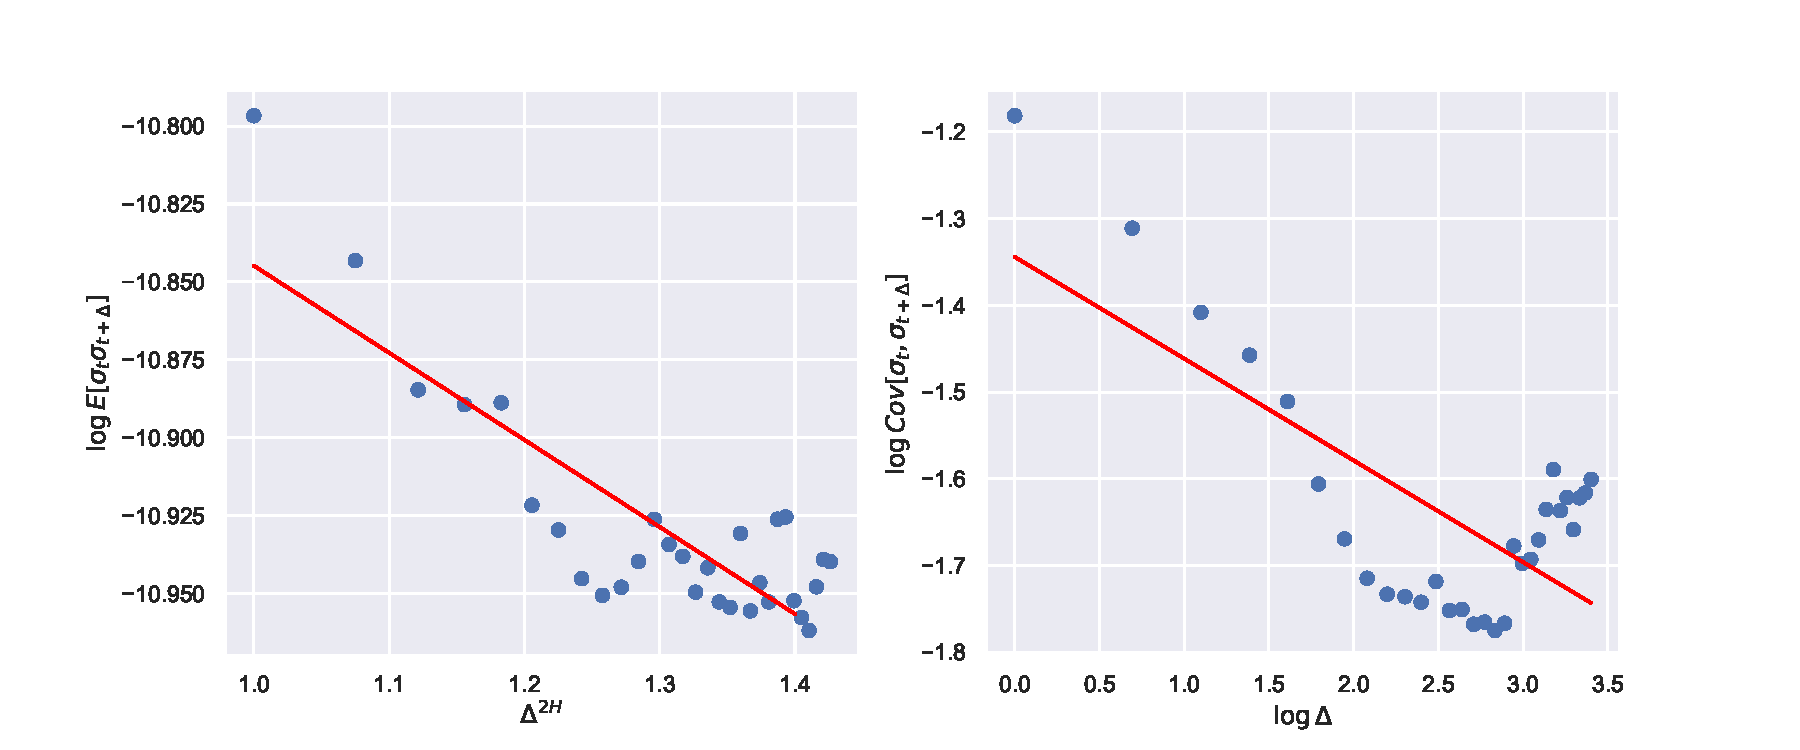
\includegraphics[width=\textwidth]{fig/YNDX RX Equity logE vs logD.pdf}
            \caption{YNDX RX Equity. Empirical counterpart of $\log\mathbb{E} \left[\sigma_{t}\sigma_{t+\Delta}\right]$ as a function of $\Delta^{2H}$ (left) and Empirical counterpart of $\log\cov [\sigma_{t}, \sigma_{t+\Delta}]$ as a function of $\log\Delta$ (right)}
        \end{figure}

    \subsection{Smoothing Effect Estimation}
        Smoothing effect is throroughly discussed in the appendix of \cite{GatheralRosenbaum2014}.

        \begin{figure}[htbp]
            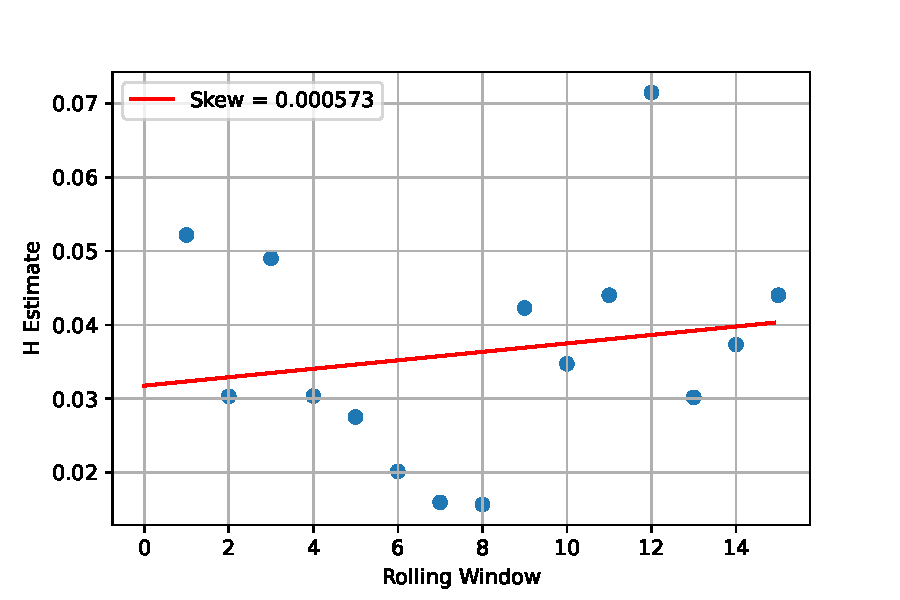
\includegraphics[width=\textwidth]{fig/YNDX RX Equity Smoothing Effect.pdf}
            \caption{YNDX RX Equity. Smoothing Effect}
            \label{fig:smooth}
        \end{figure}

        We can clearly see that due to the positive slope of the plot \ref{fig:smooth}, the hypothesis about increasing $\hat{H}$ and decreasing $\hat{\alpha}$ as $\delta$ increases is to be accepted.

    \subsection{Tests for normality of volatility's log-increments}
        In order to test the normality of the log-increments of the realized volatility, we used the following tests:
        \begin{enumerate}
            \item Visual analysis of histograms: KDE vs normal fit vs empirical fit
            \item Visual analysis of excessed kurtosis plot
            \item D'Agostino's K Squared normality test
            \item Shapiro-Wilk normality test
        \end{enumerate}

        In \cite{GatheralRosenbaum2014} the authors used \textbf{only} the visual analysis of the 
        histograms, which, as we can now say, is not surprising due to the inadequacy of results 
        for other numerical experiments.

        \subsubsection{Visual analysis of histograms and excessed kurtosis plot}
            \begin{enumerate}
                \item KDE is the \emph{kernel density estimator} of the data.
                \item \emph{Normal fit} $NF(\Delta)$ is the normal distribution fitted to the data with the same mean and variance.
                \item \emph{Empirical fit} $EF(\Delta)$ is the scaled normal distribution:
                    \begin{itemize}
                        \item $EF(1)$ is said to be same as the $NF(1)$
                        \item $EF(\Delta)$ for $\Delta > 1$ is said to be a scaled $NF(1)$ by the 
                            factor of $\Delta^{\hat{H}}$ (by this we test the monofractal scaling 
                            property of normal distribution)
                    \end{itemize}
            \end{enumerate}

            \begin{figure}[htbp]
                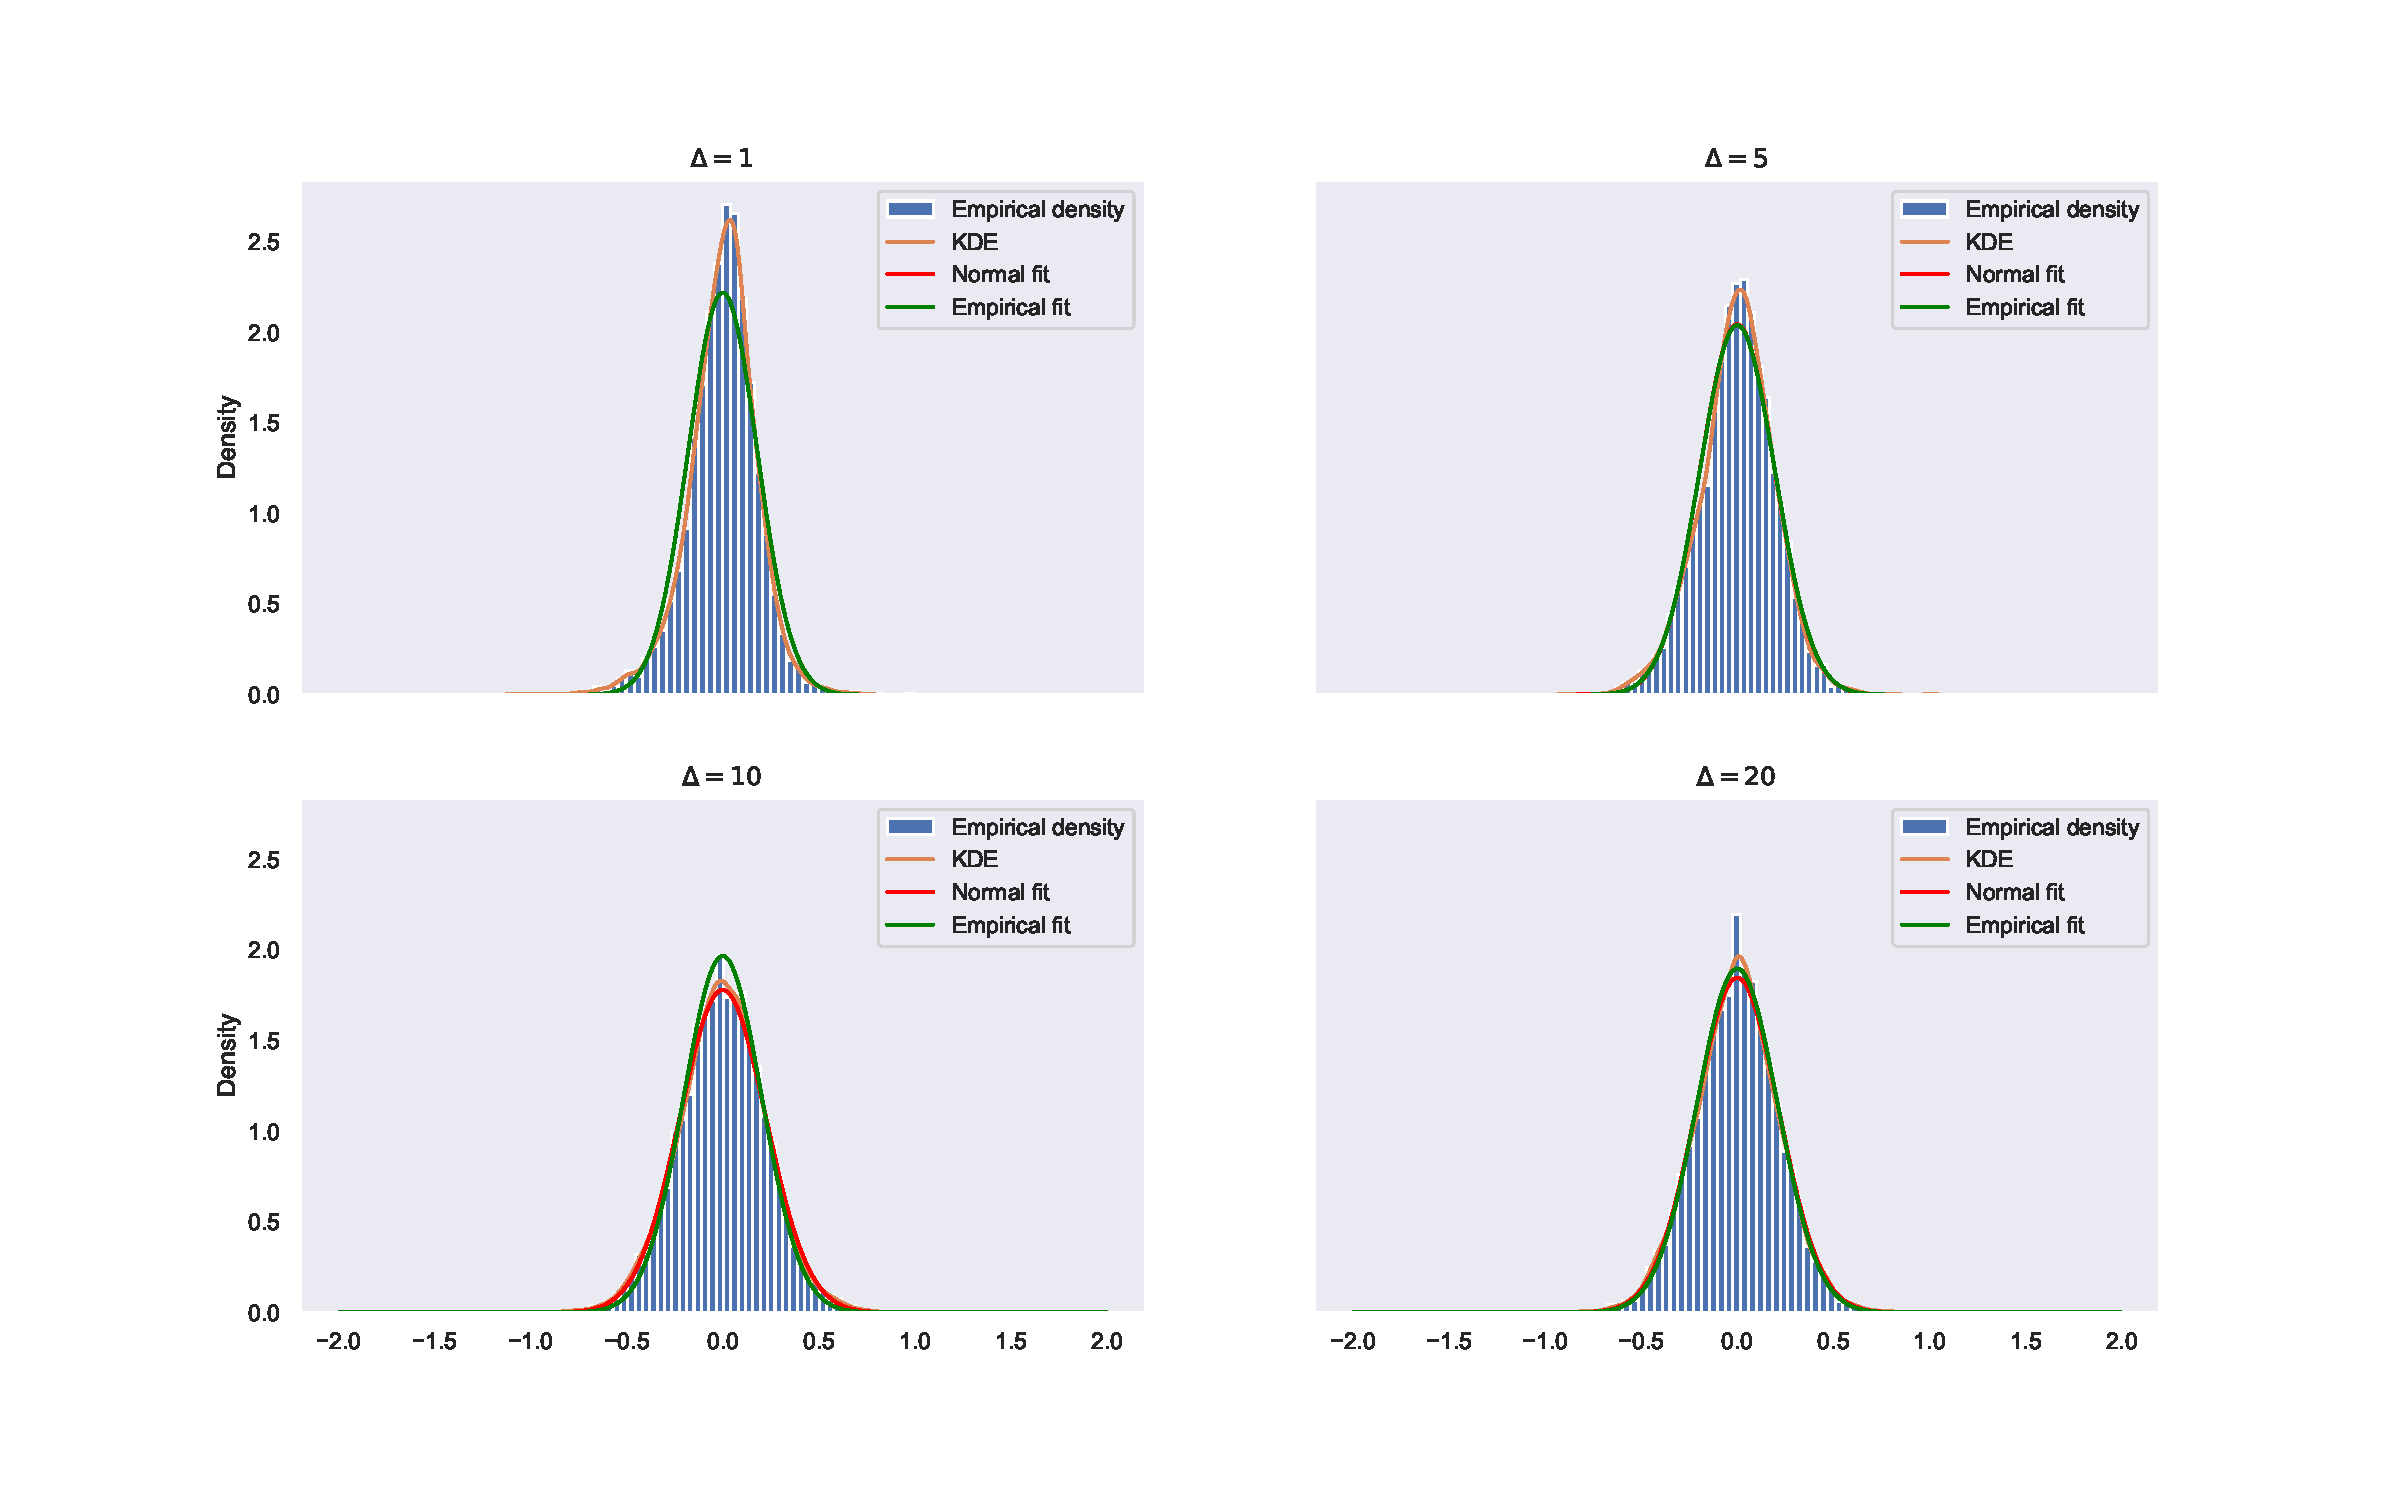
\includegraphics[width=\textwidth]{fig/YNDX RX Equity 30 Lag Hists.pdf}
                \caption{YNDX RX Equity. Empirical density of $\log \sigma_{t+\Delta} - \log \sigma_{t}$ for $\Delta = 1, 5, 10, 20$ days.}
                \label{fig:lagHists}
            \end{figure}

            Looking at the figure \ref{fig:lagHists}, we may form a conclusion: $KDE$ and $EF$ are a decent normality approximations 
            for $\Delta = 10, 20$. For others, we don't get a fancy picture: $KDE(1)$ and $KDE(5)$ have a large kurtosis 
            (they are too 'peaky' for them to be normally distributed). 
            Excessed curtosis plot \ref{fig:exkurt} confirms our visual conclusion for $KDE$ and $EF$ plots.

            \begin{figure}[htbp]
                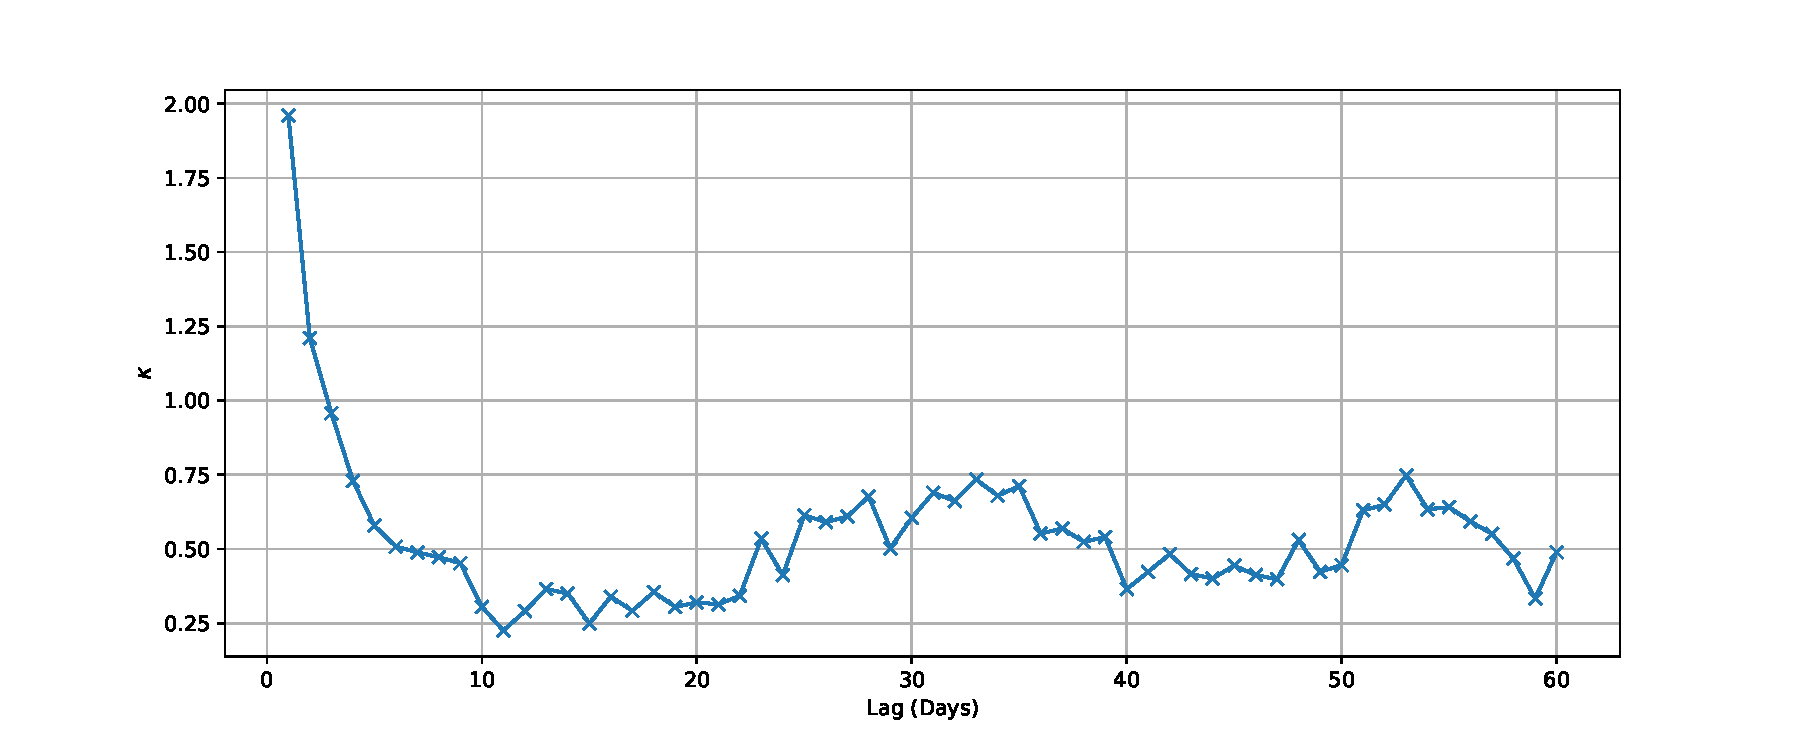
\includegraphics[width=\textwidth]{fig/YNDX RX Equity Excessed Curtosis.pdf}
                \caption{YNDX RX Equity. Excessed kurtosis $\kappa$ as a function of $\Delta$}
                \label{fig:exkurt}
            \end{figure}


        \subsubsection{Statistical tests for normality}
            We fix the confidence level to be $\alpha = 0.05$.
            \begin{nb}
                Both of these tests require the data to be independent, but we cannot guarantee this 
                due to the dependence of fBm's increments. We do our best to analyse the population,
                but these two tests give us weak proof of normality due to possible correlations.
            \end{nb}

            Looking at the tables with the results of Shapiro-Wilk and D'Agostino's K-Squared tests 
            (tables \ref{tab:normality_tests_YNDX_RX} -- \ref{tab:normality_tests_LKOD_LI}), we can see that for the majority of lags and for the 
            majority of the considered assets, both tests showed the result "Not normal", i.e. both tests
            rejected the null hypothesis. 

            \
            
            \noindent The three possible explanations are:
            \begin{enumerate}
                \item The tests are correct and the data is not normally distributed or is correlated strongly.
                \item The visual analysis of the histograms show that for many lags the KDE plot, the normal fit and 
                the empirical fit are very similar, therefore, the distribution is normal, but the data is 
                correlated strongly. The excessed kurtosis plot shows that the data is distributed very close to the normal
                distribution for $\Delta > 5$, and at its closest distance for $\Delta \in [10, 22]$.
                \item We get a population sampling error (not enough data).
            \end{enumerate} 

    \chapter{Modelless Estimation of Roughness}

        \section{Sample normalized variation as a measure of roughness}
    \subsection{Theoretical parameters}
        Let us consider a sequence of partitions $\pi^n$ of $\left[0, T\right]$ with 
        $\left|\pi^n\right|:=\max_{t_i^n \in \pi^n} (t_{i+1}^n - t_i^n) \to 0$. 
        \begin{definition}
            A function $x \in C[0, T]$ is said to have the finite $p$-th variation along the sequence of partitions $\pi^n$ 
            if there exists a continious increasing function $\left[x\right]_{\pi}^{(p)}$ such that for all subpartitions $\tilde\pi^n(t) = \pi^n \cap [0, t]$
            \begin{equation}
                \sum_{t_i^n \in \tilde\pi^n(t)} \left|x(t_{i+1}^n) - x(t_i^n)\right|^p \to \left[x\right]_{\pi}^{(p)}(t), \quad n\to \infty,
            \end{equation}
            and the set of all functions having finite $p$-th variation along $\pi$ we denote $V_\pi^p$.
        \end{definition}
        \begin{definition}
            The \emph{variation index} of a path $x$ is defined as $p^\pi(x) := \inf \left\{p\geq 1 \colon \quad x\in V_\pi^p\right\}$, and the \emph{roughness index} is defined as $H^\pi(x):=\frac{1}{p^\pi(x)}$.
        \end{definition}
        It has been proven that for fBm with Hurst parameter $H$ $p^\pi(W^H) = \frac{1}{H}$ and $H^\pi(W^H) = H$.
        
        \begin{definition}
            $x\in V_\pi^p$ is said to have $p$-th normalized variation if there exists such continious function $w(x, p, \pi)\colon [0, T] \to \mathbb{R}$ that
            \begin{equation}
                \sum_{\tilde\pi^n(t)}\frac{\left|x(t_{i+1}^n) - x(t_i^n)\right|^p}{\left[x\right]_{\pi}^{(p)}(t_{i+1}^n)-\left[x\right]_{\pi}^{(p)}(t_i^n)} (t_{i+1}^n-t_{i}^n) \to w(x, p, \pi).
            \end{equation}
        \end{definition}

        From Theorem 2.4 \cite{Cont2022}, it is known that the variation index must be found as a solution of 
        \begin{equation}
            w(x, p, \pi) = t.
        \end{equation}
    \subsection{The $W$ Statistic}
        \begin{figure}[htbp]
            \centering
            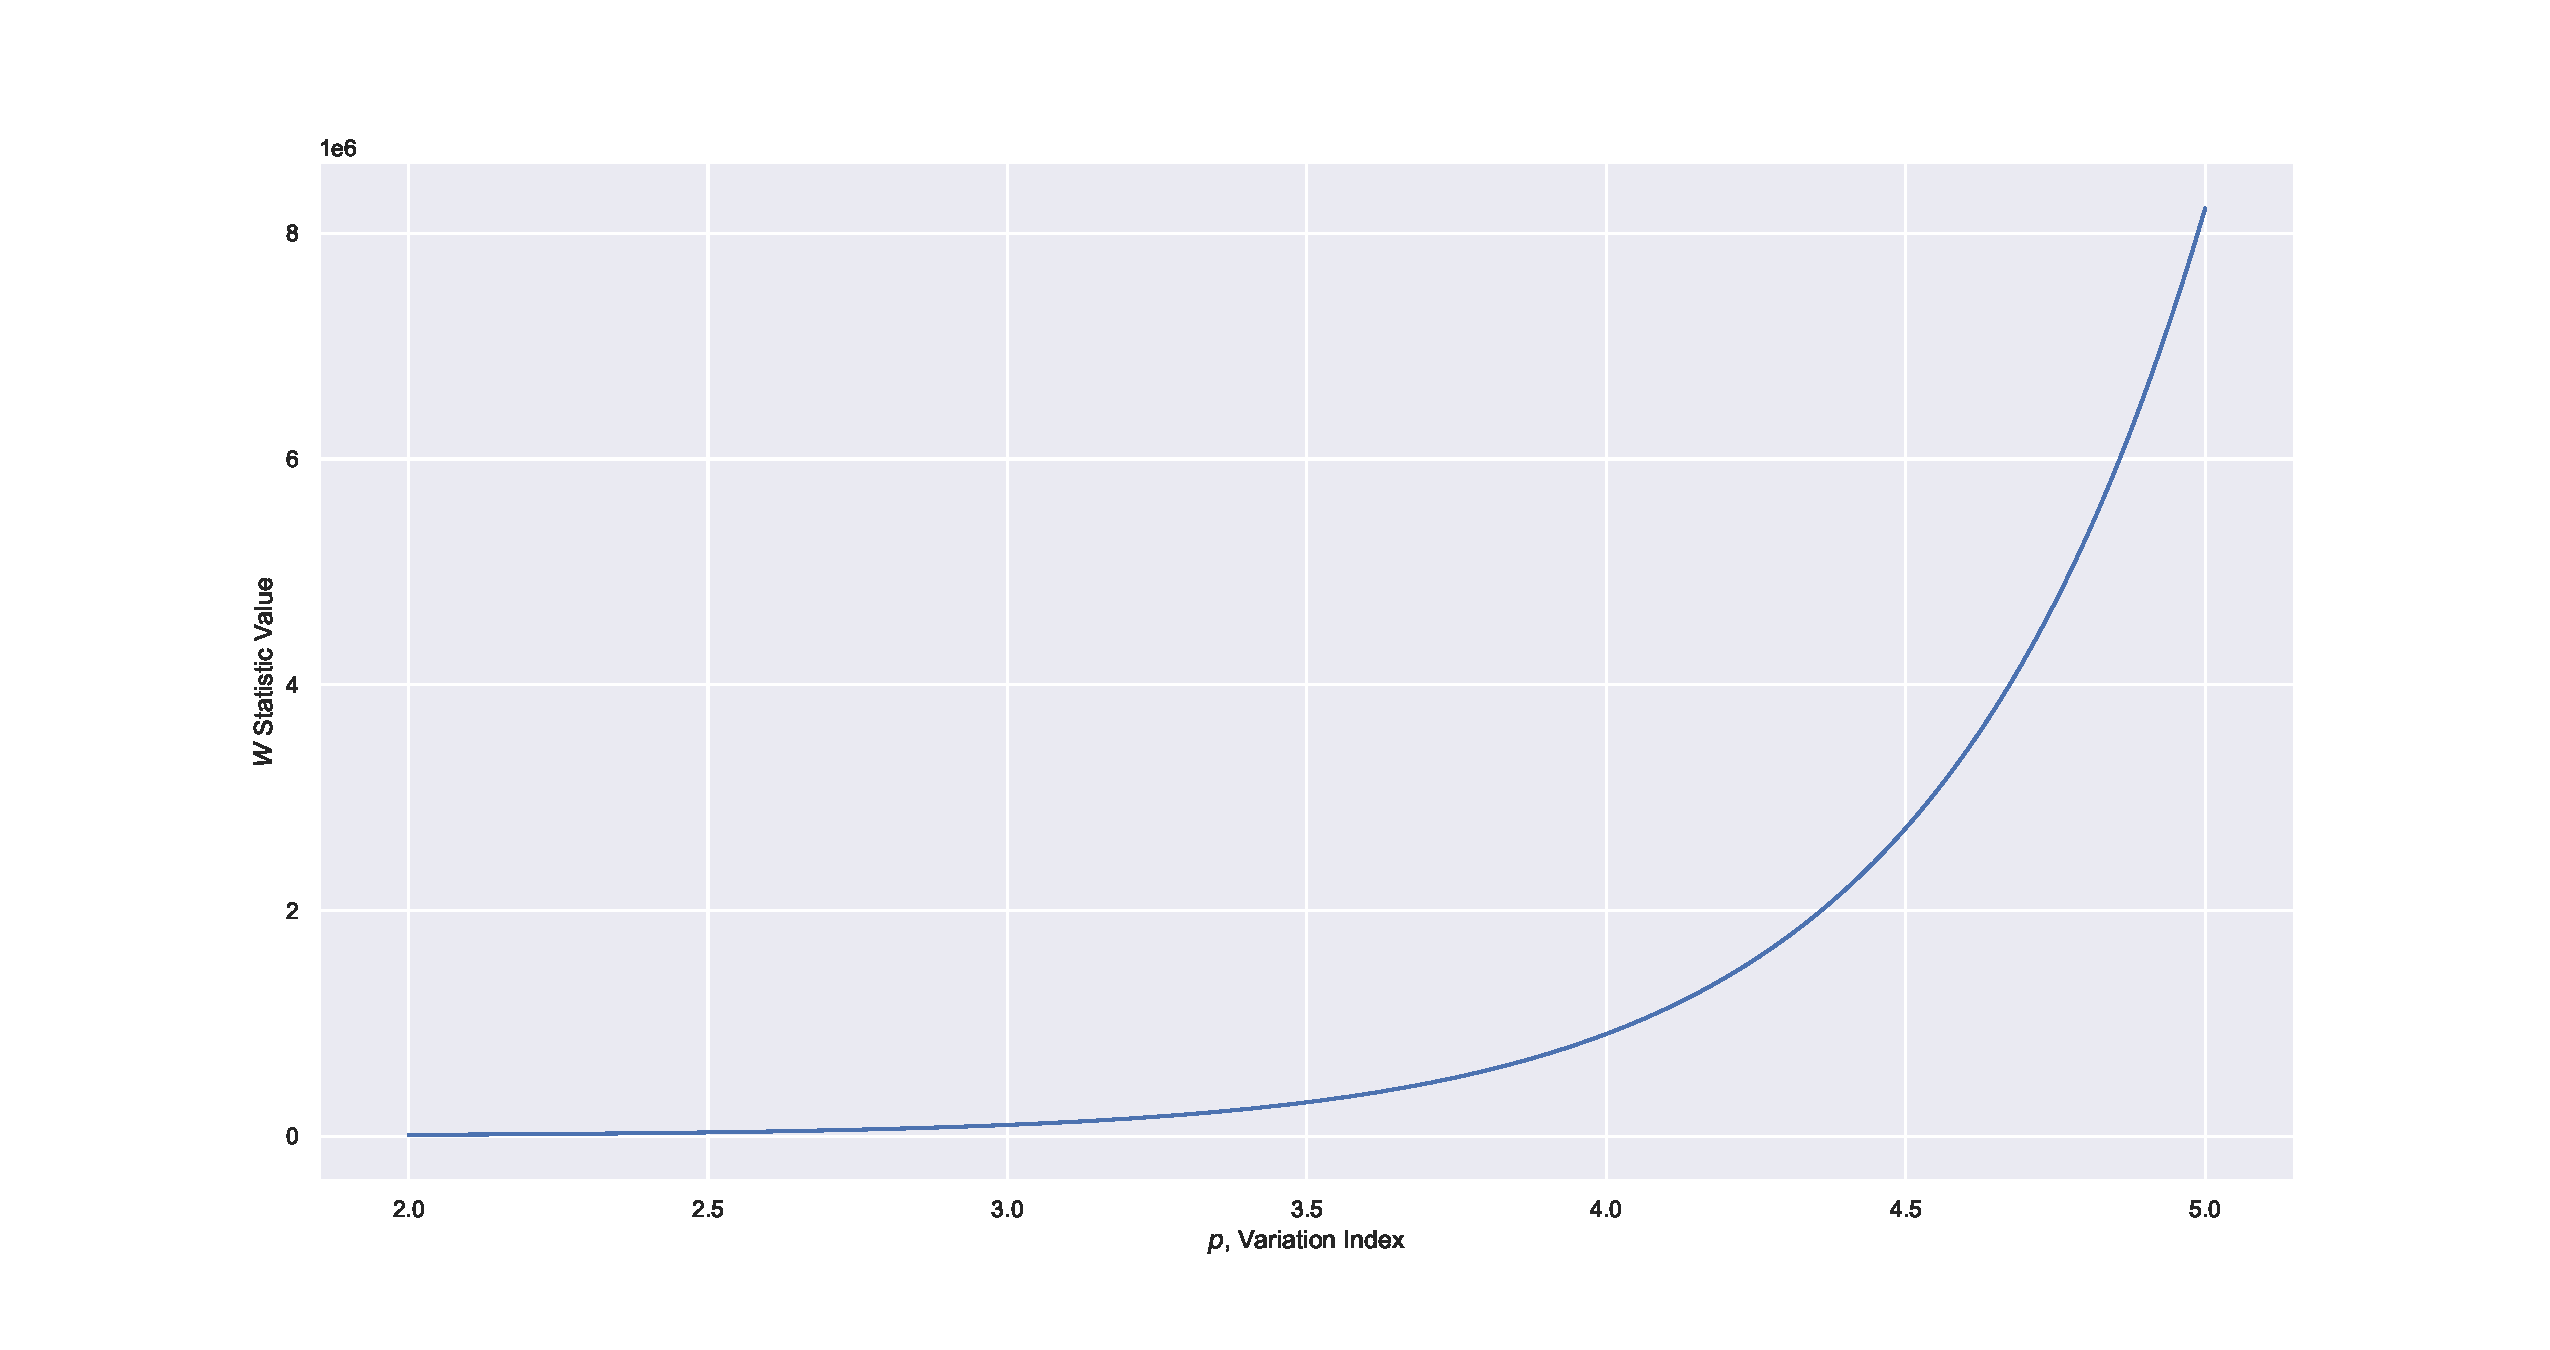
\includegraphics[width=\linewidth]{fig/W Stat Illustration.pdf}
            \caption{The $W$ statistic illustration as a function of $p$}
        \end{figure}

\section{Roughness estimation of Monte-Carlo simulations}

    \subsection{Brownian and fractional Brownian motion}
        We shall test our method on those processes, whose roughness is well-known.
        \subsubsection{Brownian motion}
            \begin{figure}[htbp]
                \centering
                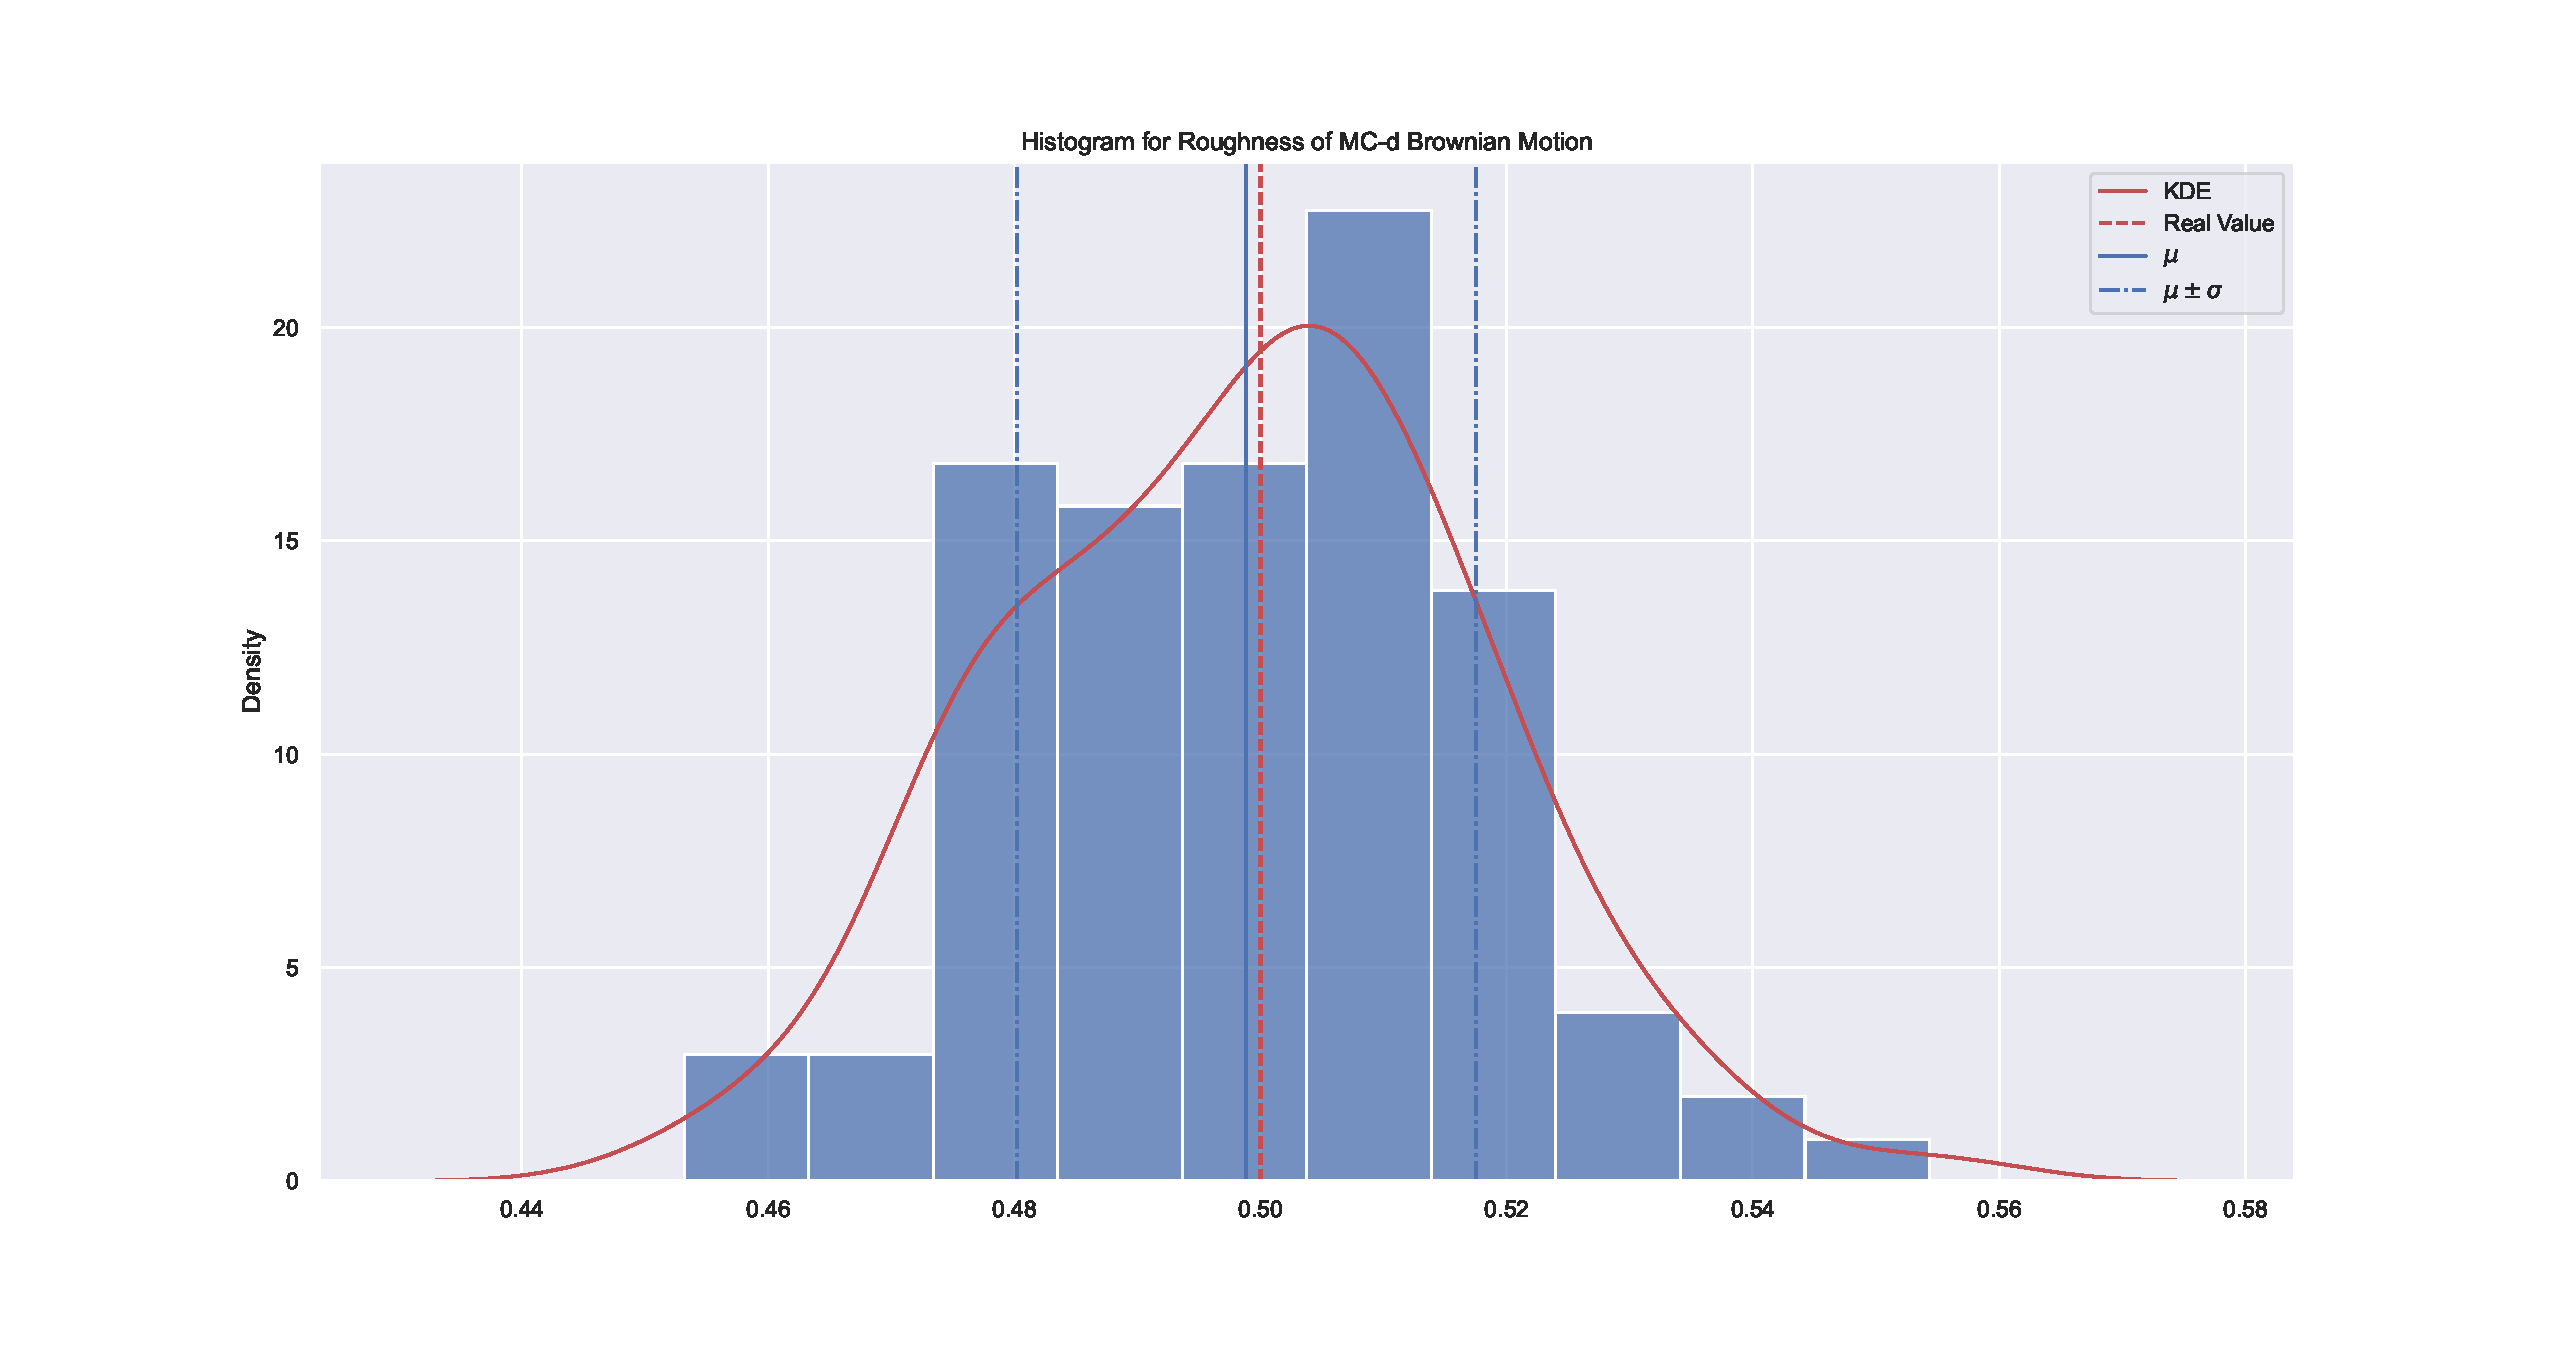
\includegraphics[width=\linewidth]{fig/Histogram for Roughness of MC-d Brownian Motion.pdf}
                \caption{Histogram for roughness of Brownian motion}
            \end{figure}

            We observe that the roughness index is equal to $0.4988$, which is a pretty good approximation.

        \subsubsection{Fractional Brownian motion (Davies-Harte method)}
            We considered four Hurst parameters for simulation: $0.15$, $0.35$, $0.55$, and $0.75$. We used the Davies-Harte method of generating 
            the fBm since this one is widely accepted as the most precise. We observe not the best approcsimations, but they are decent enough to be in $(\mu-\sigma, \mu+\sigma)$.
            \begin{figure}[htbp]
                \centering
                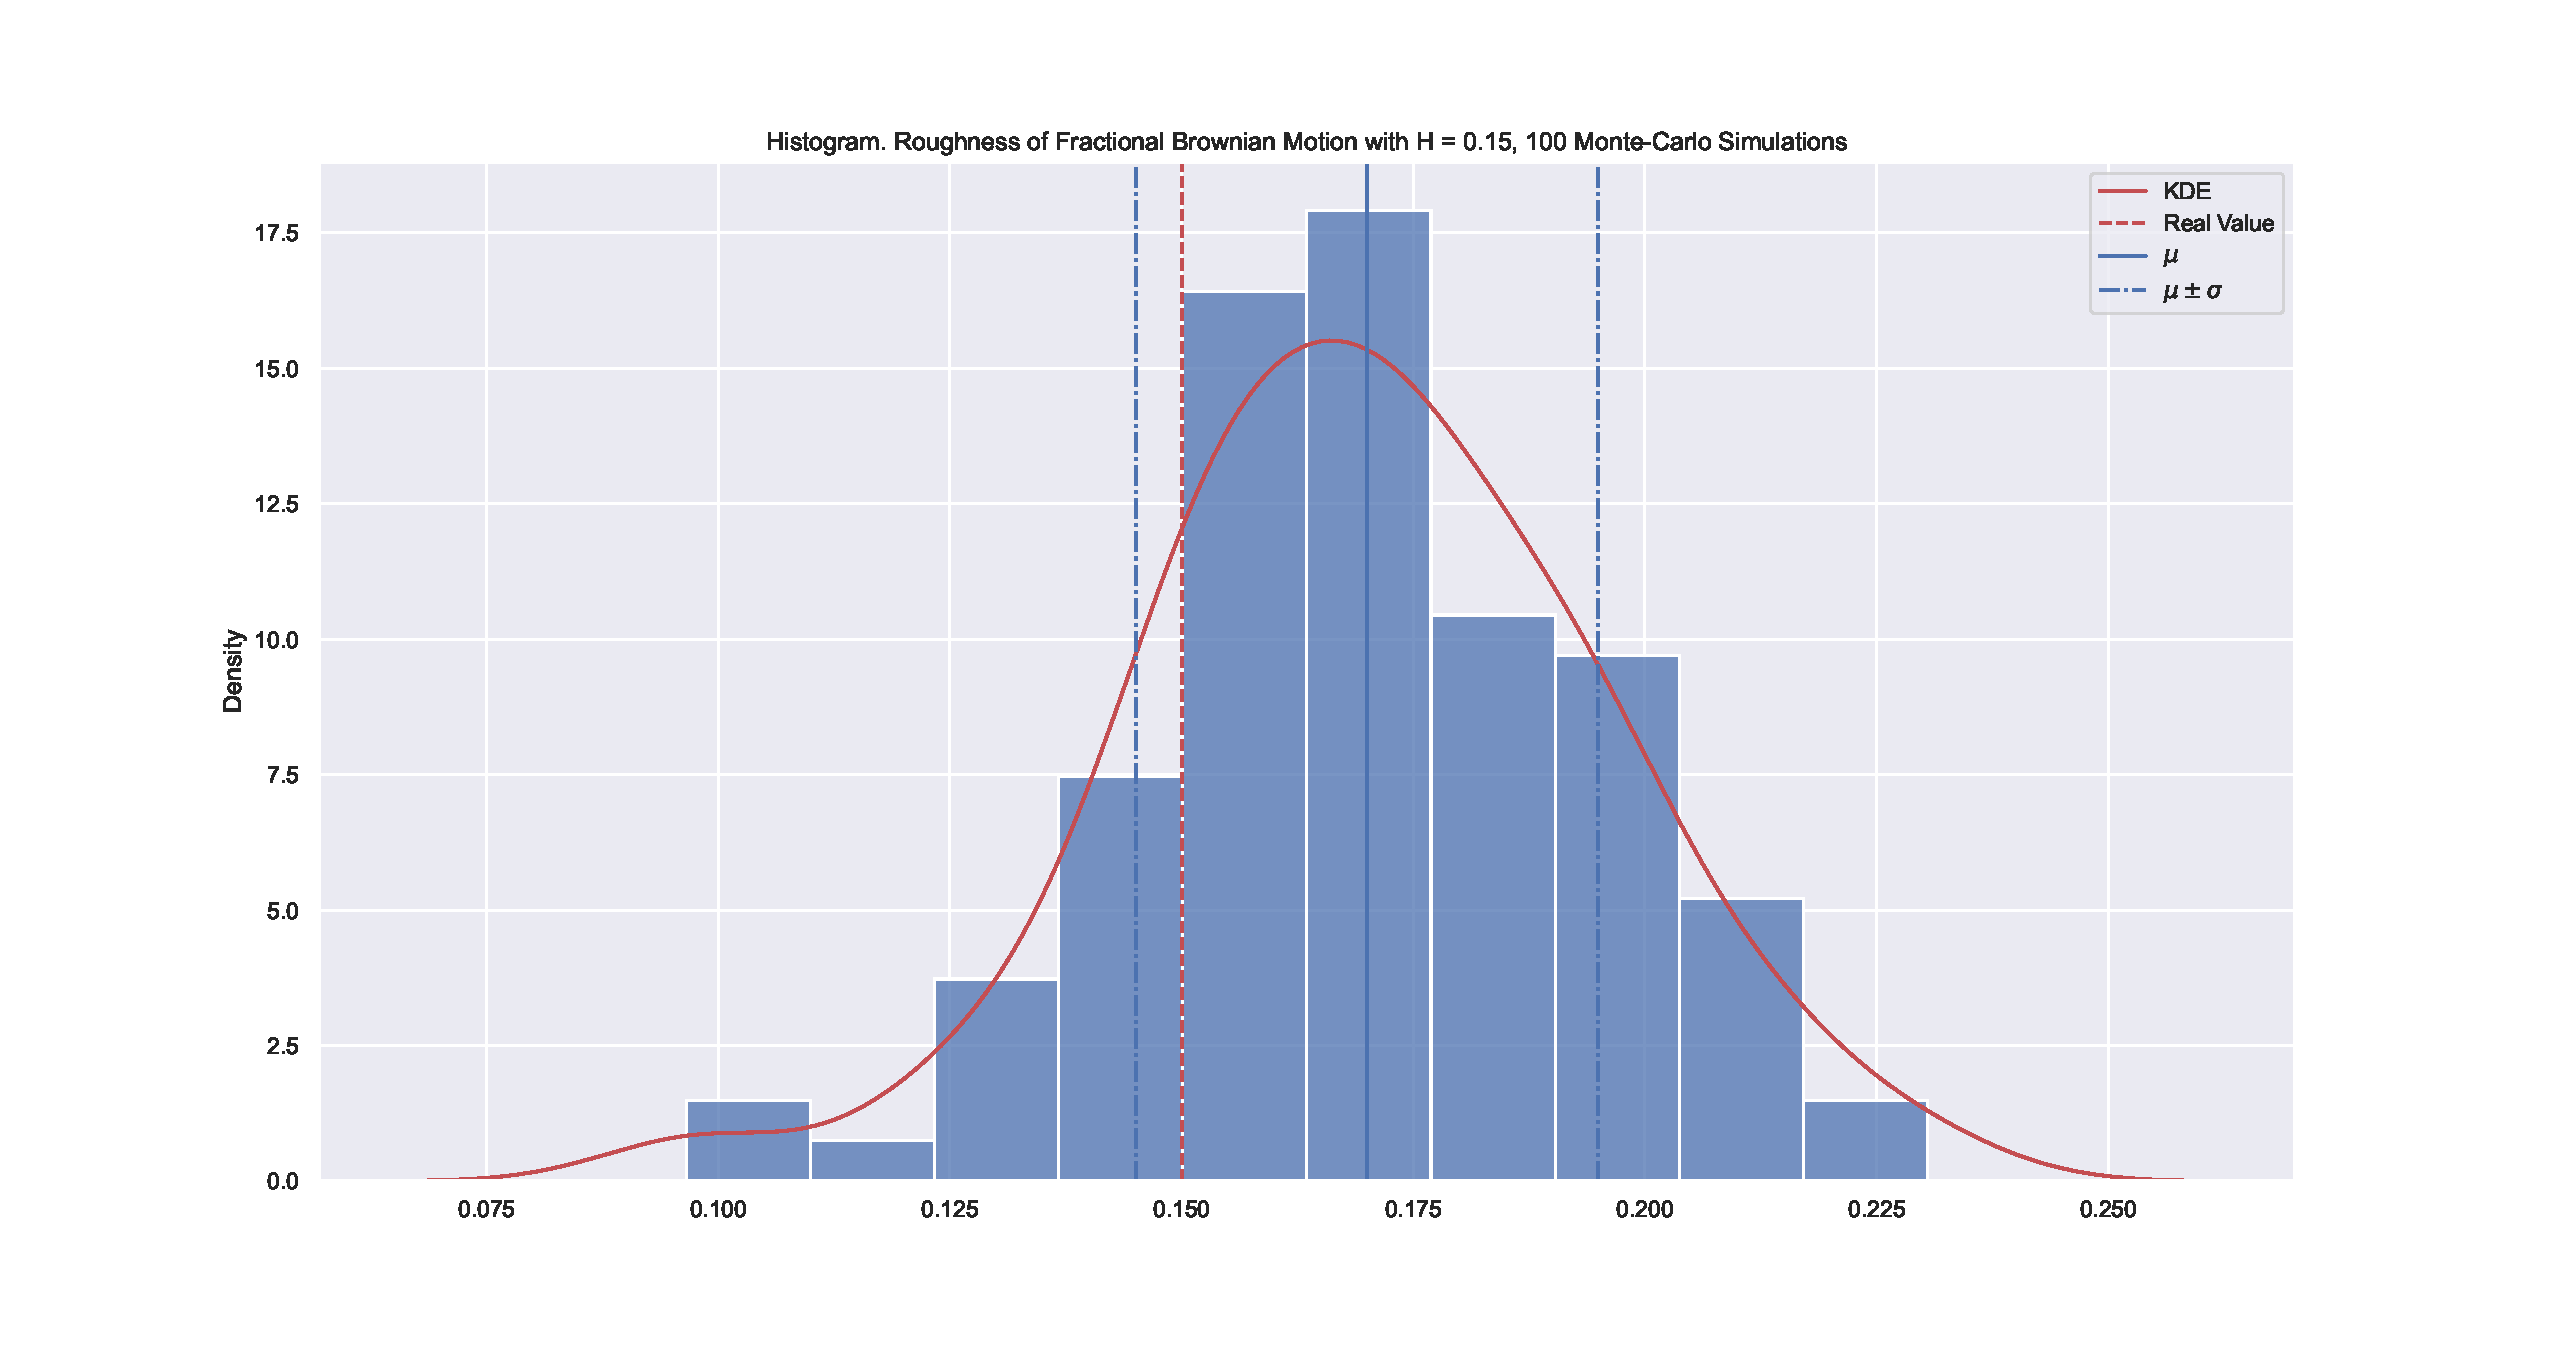
\includegraphics[width=\linewidth]{fig/Histogram. Roughness of Fractional Brownian Motion with H = 0.15, 100 Monte-Carlo Simulations.pdf}
                \caption{Histogram for roughness of fractional Brownian motion}
            \end{figure}
            \begin{figure}[htbp]
                \centering
                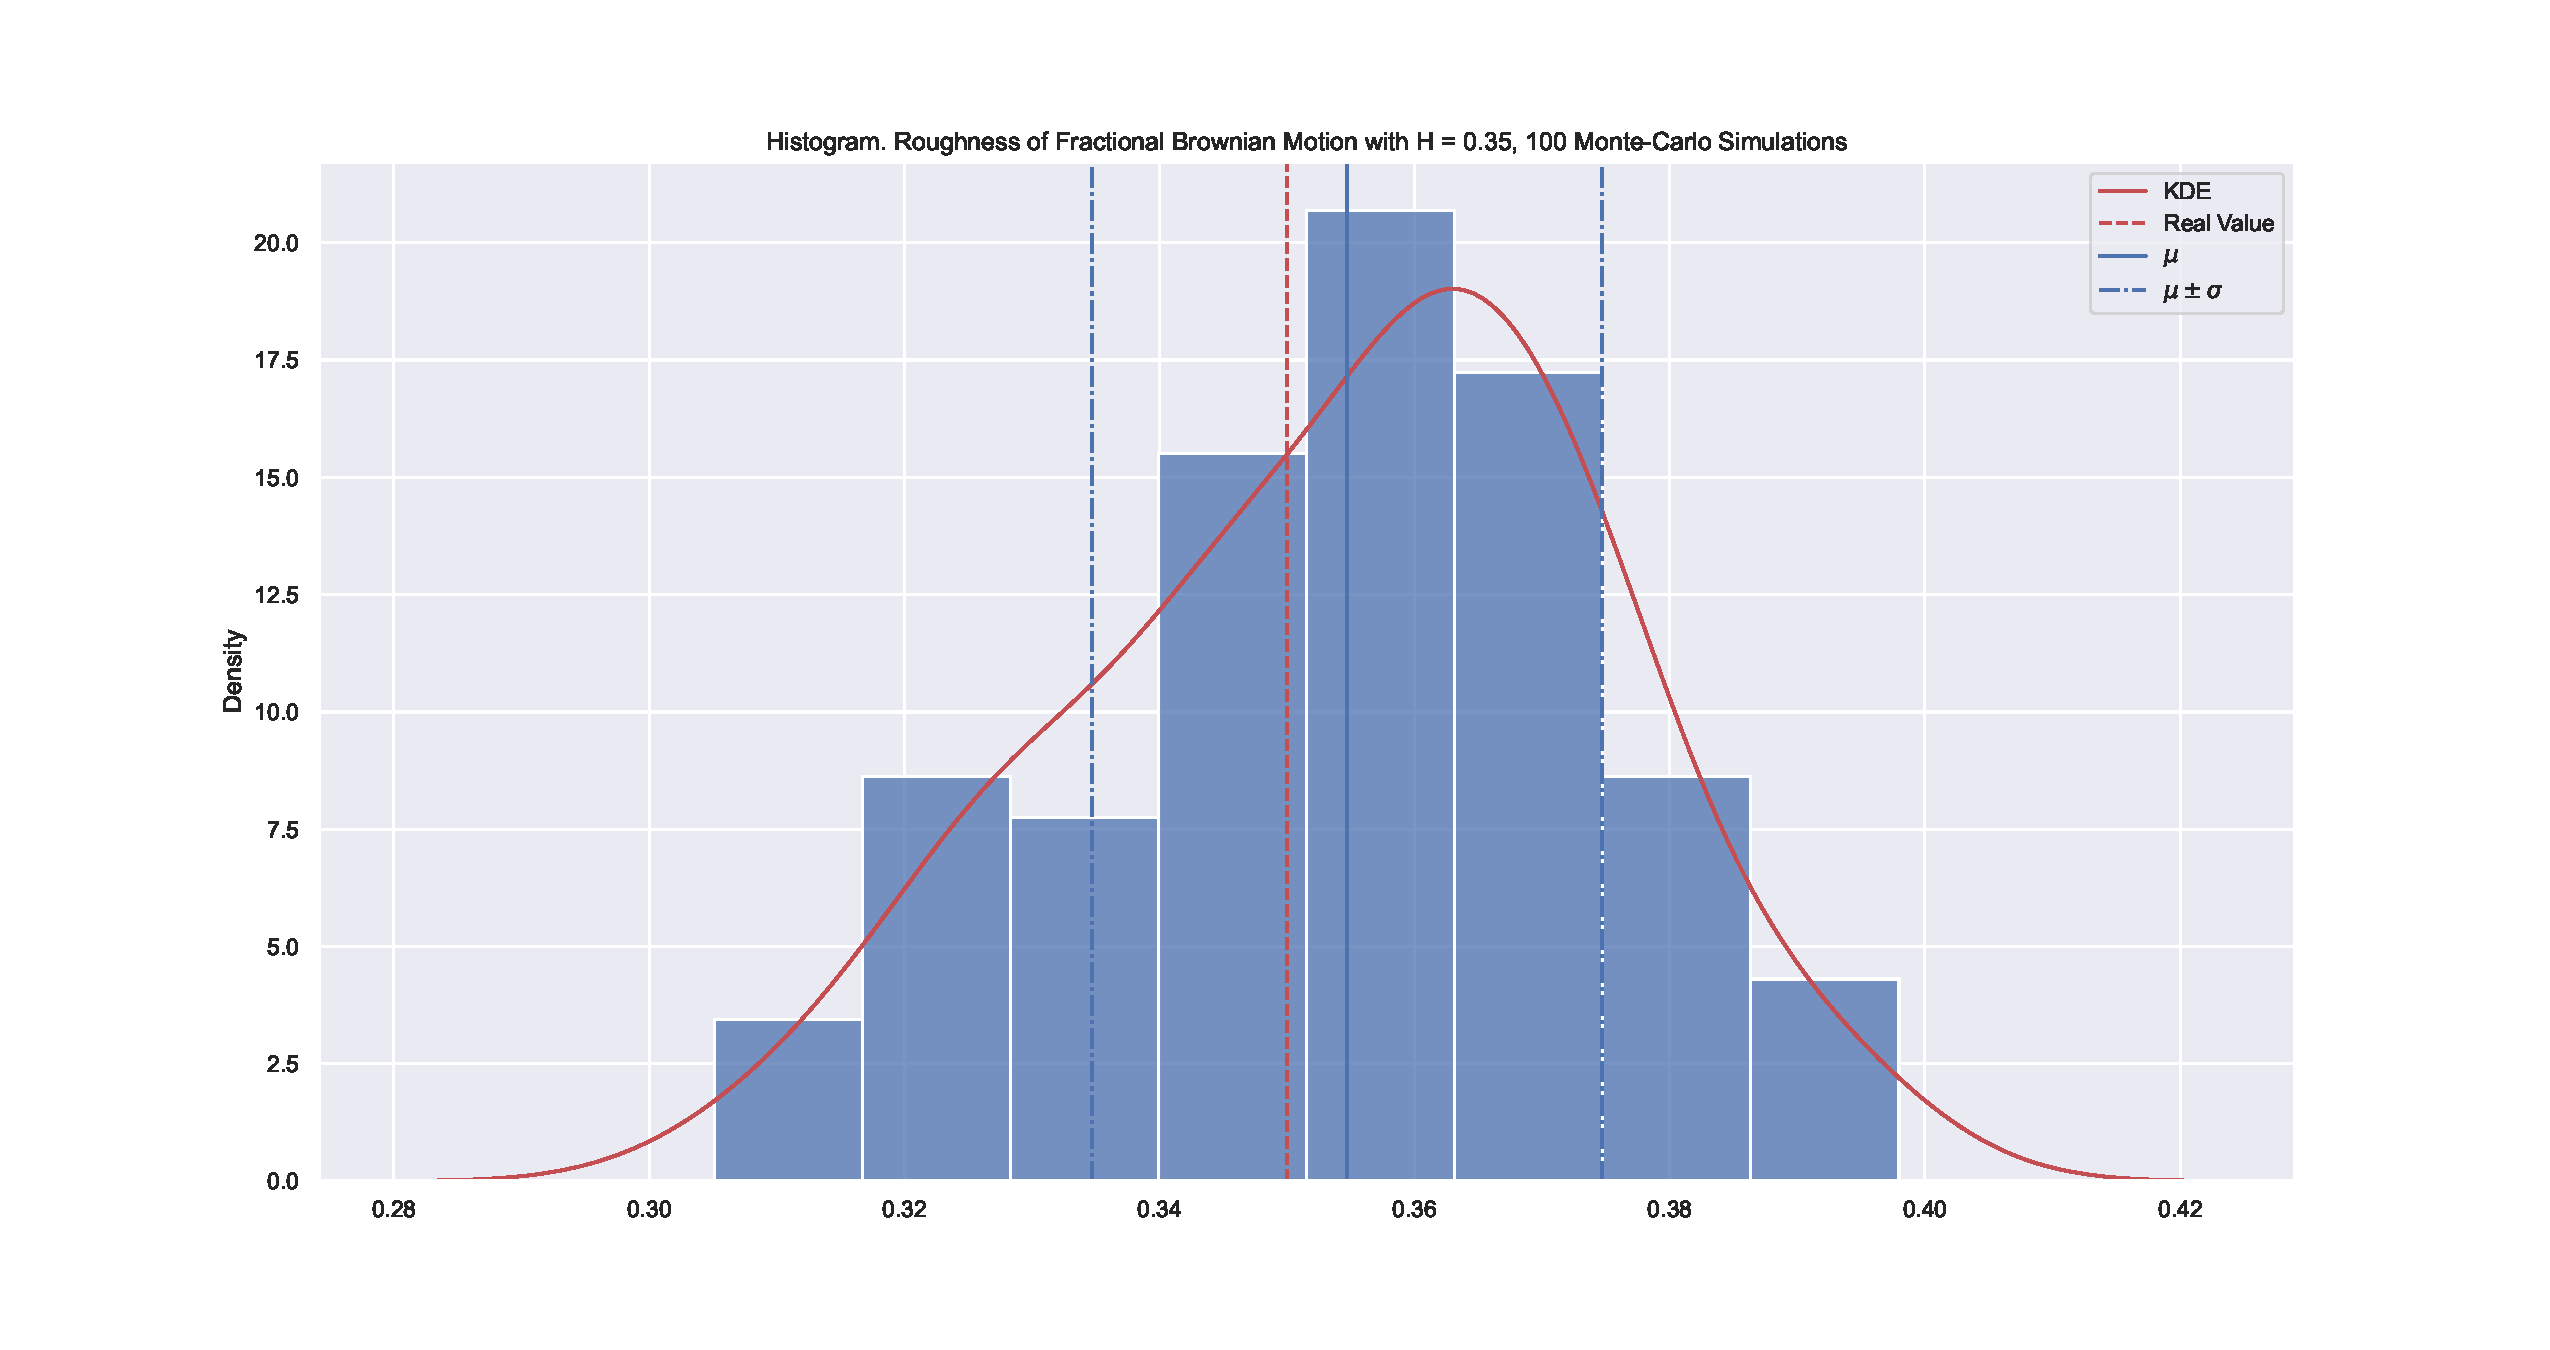
\includegraphics[width=\linewidth]{fig/Histogram. Roughness of Fractional Brownian Motion with H = 0.35, 100 Monte-Carlo Simulations.pdf}
                \caption{Histogram for roughness of fractional Brownian motion}
            \end{figure}
            \begin{figure}[htbp]
                \centering
                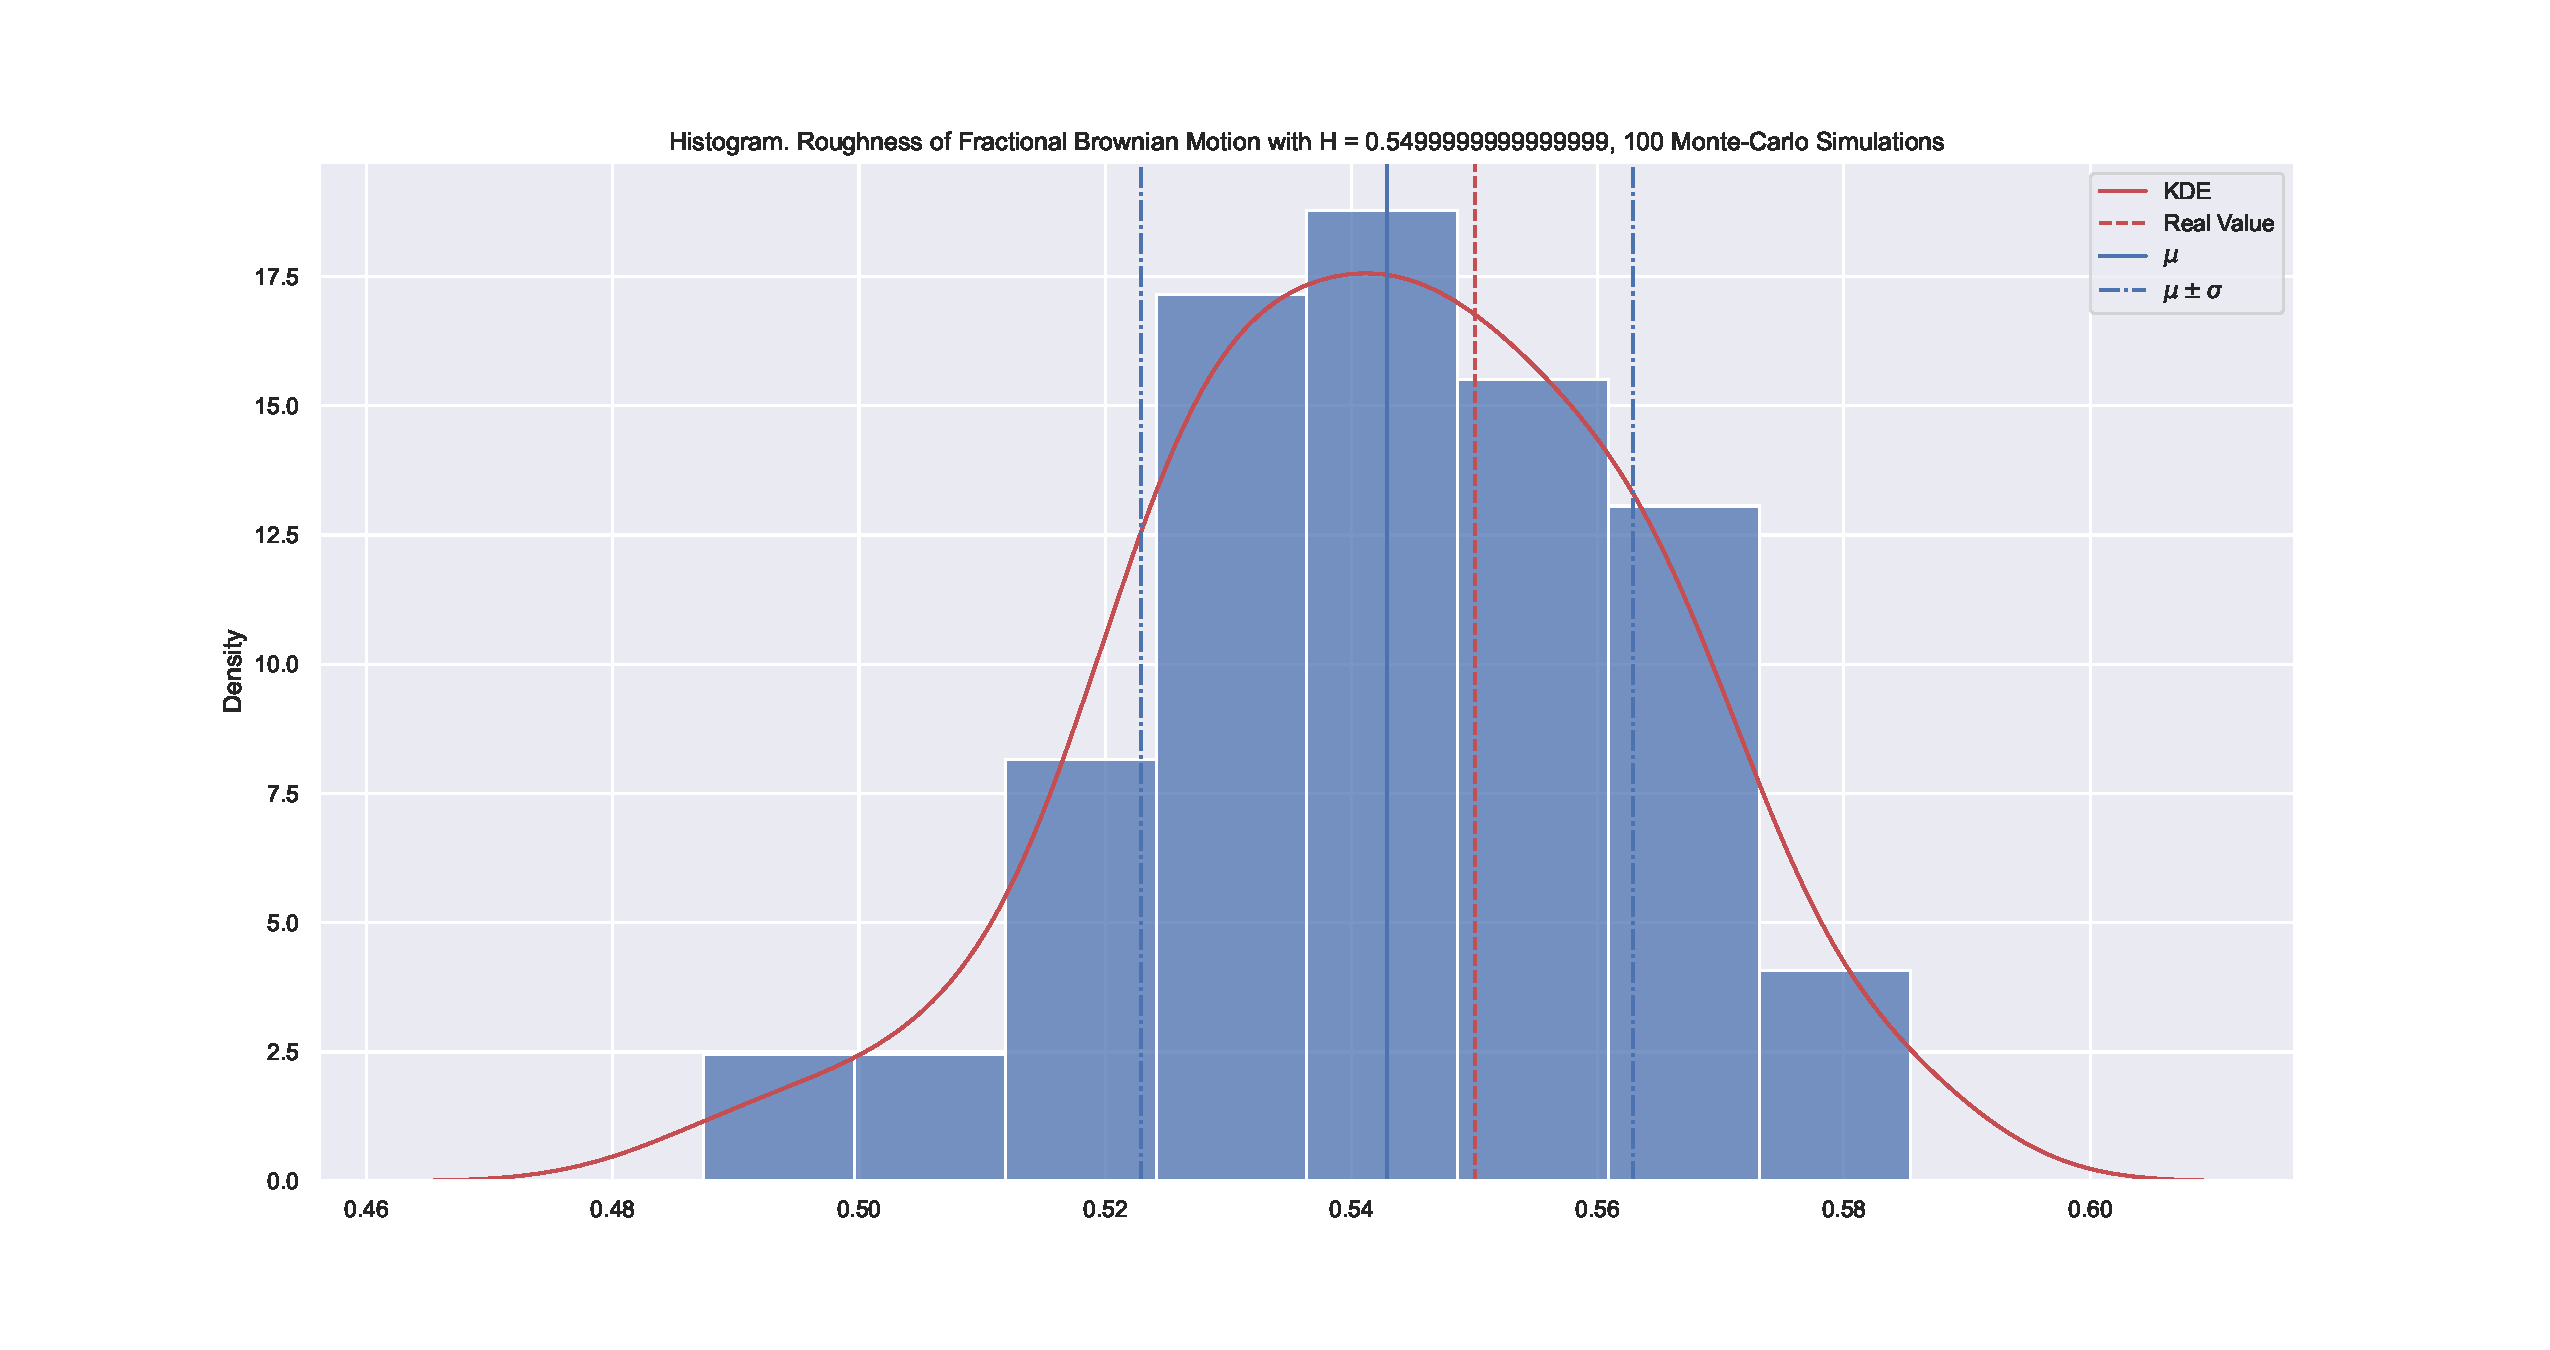
\includegraphics[width=\linewidth]{fig/Histogram. Roughness of Fractional Brownian Motion with H = 0.55, 100 Monte-Carlo Simulations.pdf}
                \caption{Histogram for roughness of fractional Brownian motion}
            \end{figure}
            \begin{figure}[htbp]
                \centering
                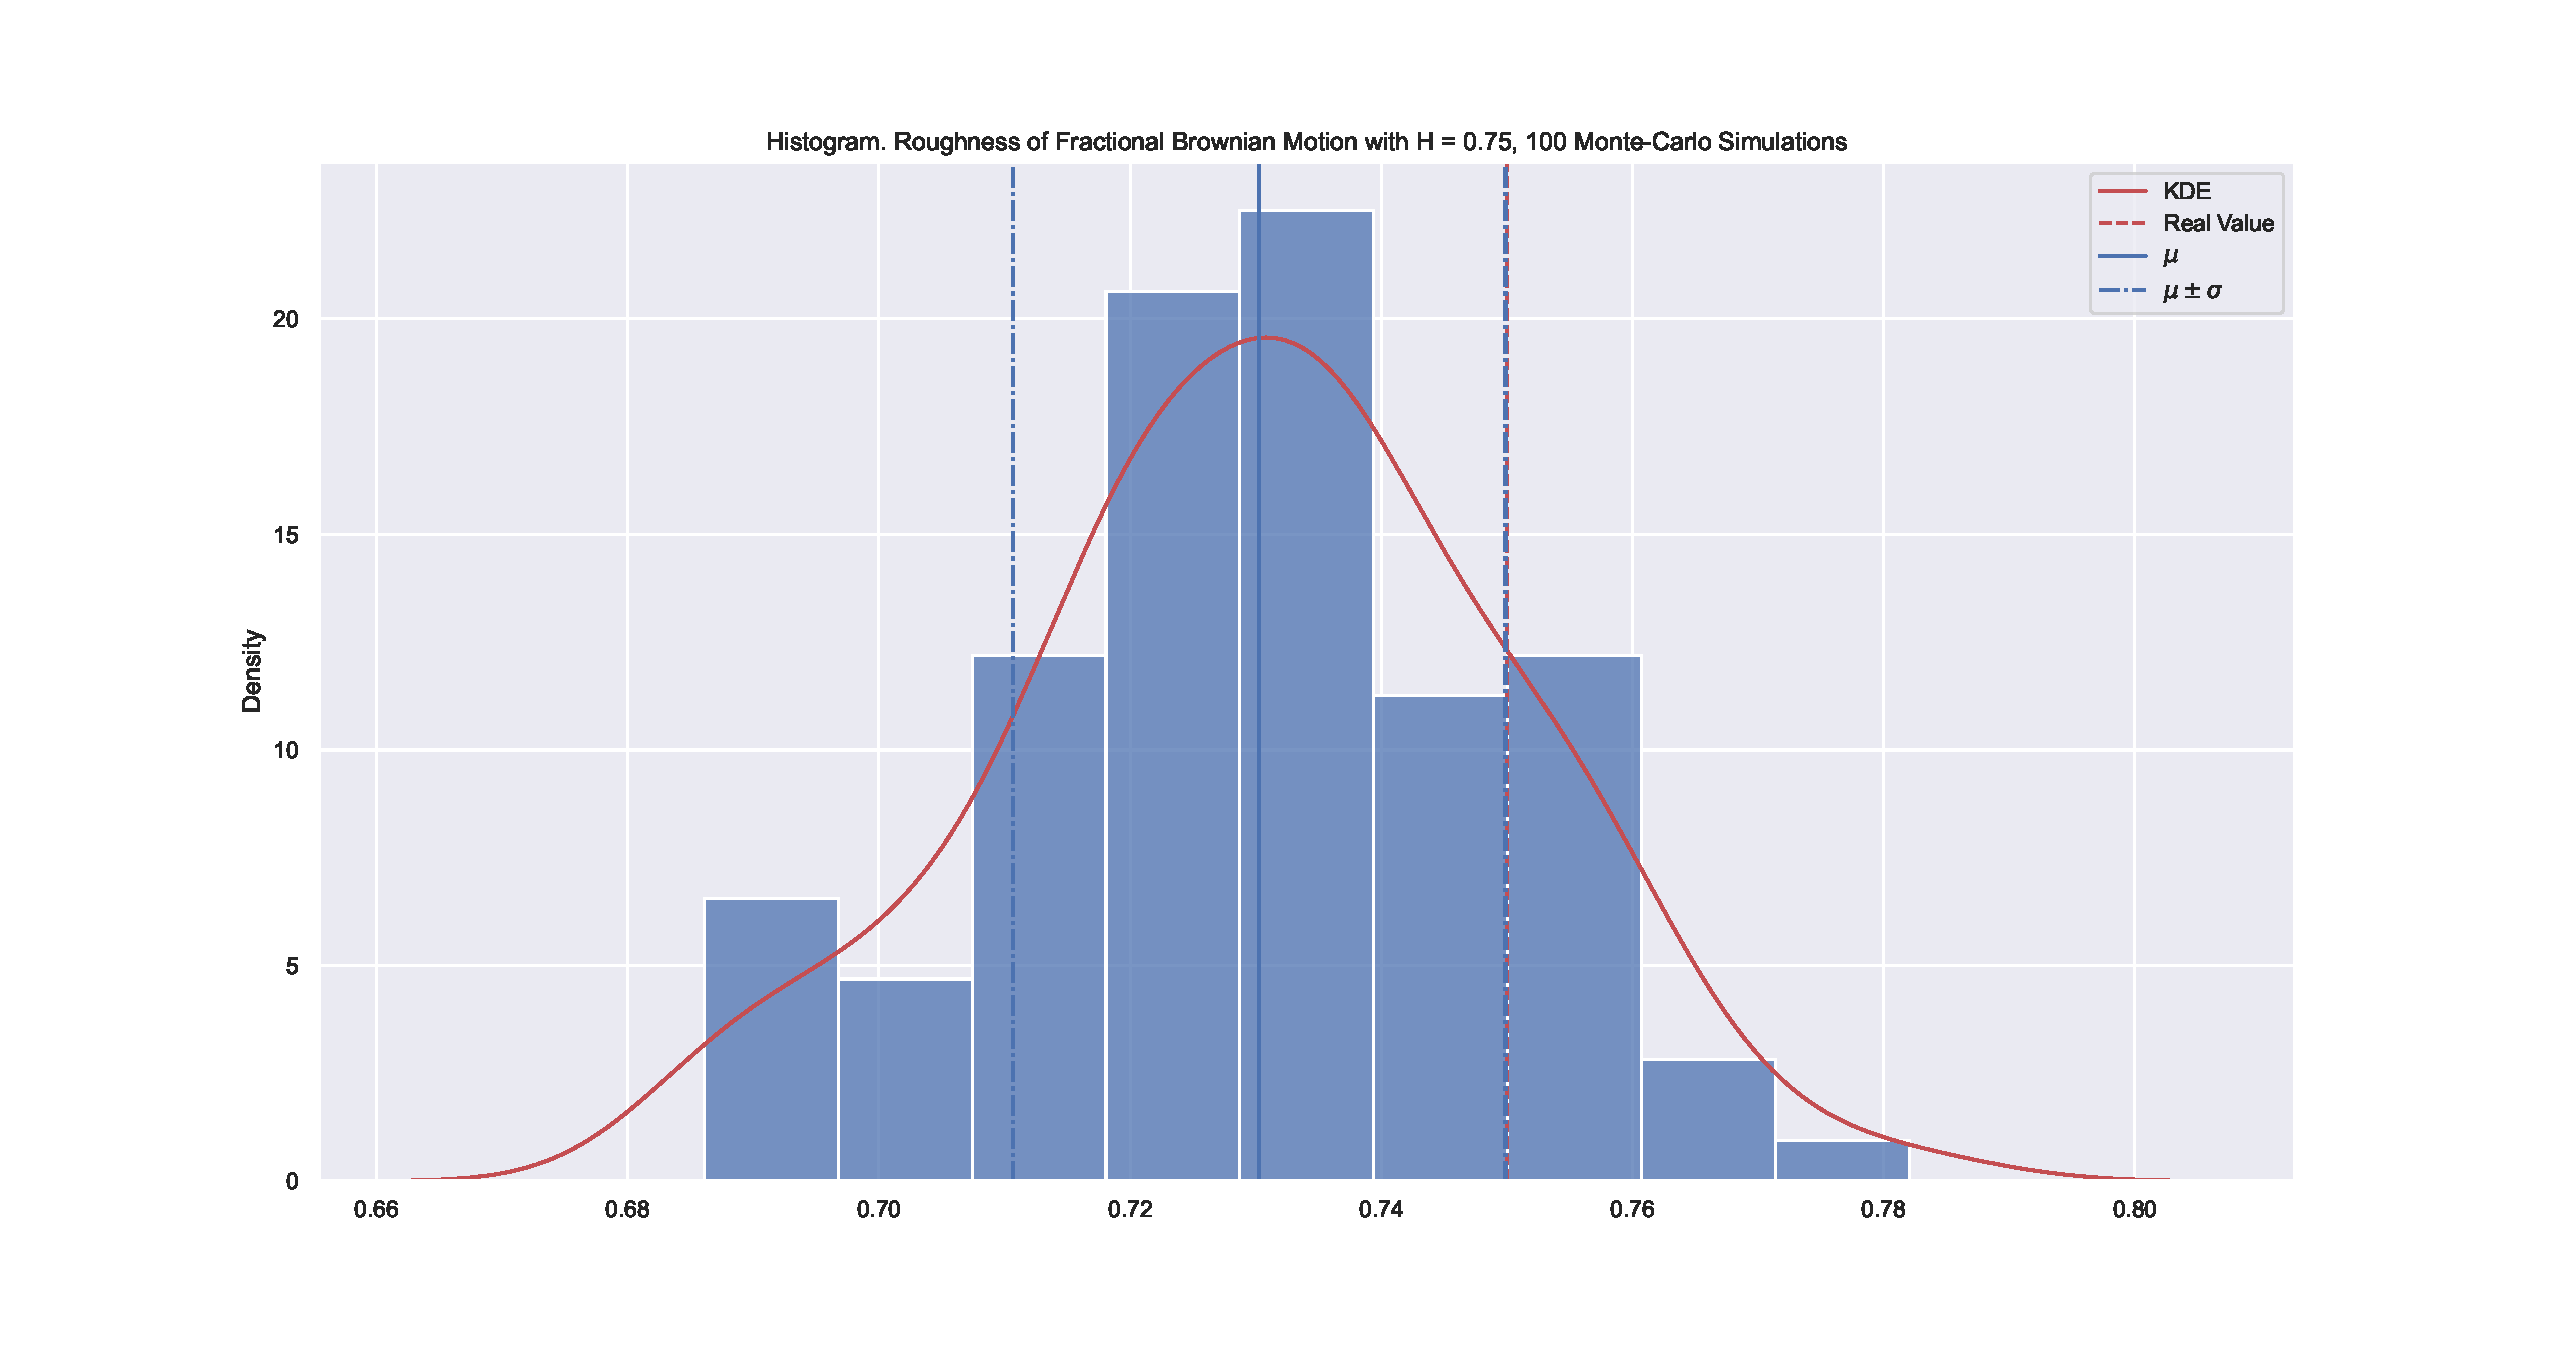
\includegraphics[width=\linewidth]{fig/Histogram. Roughness of Fractional Brownian Motion with H = 0.75, 100 Monte-Carlo Simulations.pdf}
                \caption{Histogram for roughness of fractional Brownian motion}
            \end{figure}

   \subsection{Heston stochastic volatility model}
        We observe that roughness estimations for instantaneous volatiltity and realized volatility significantly differ, which was described in the article for fOU processes.
    
    \begin{figure}[htbp]
        \centering
        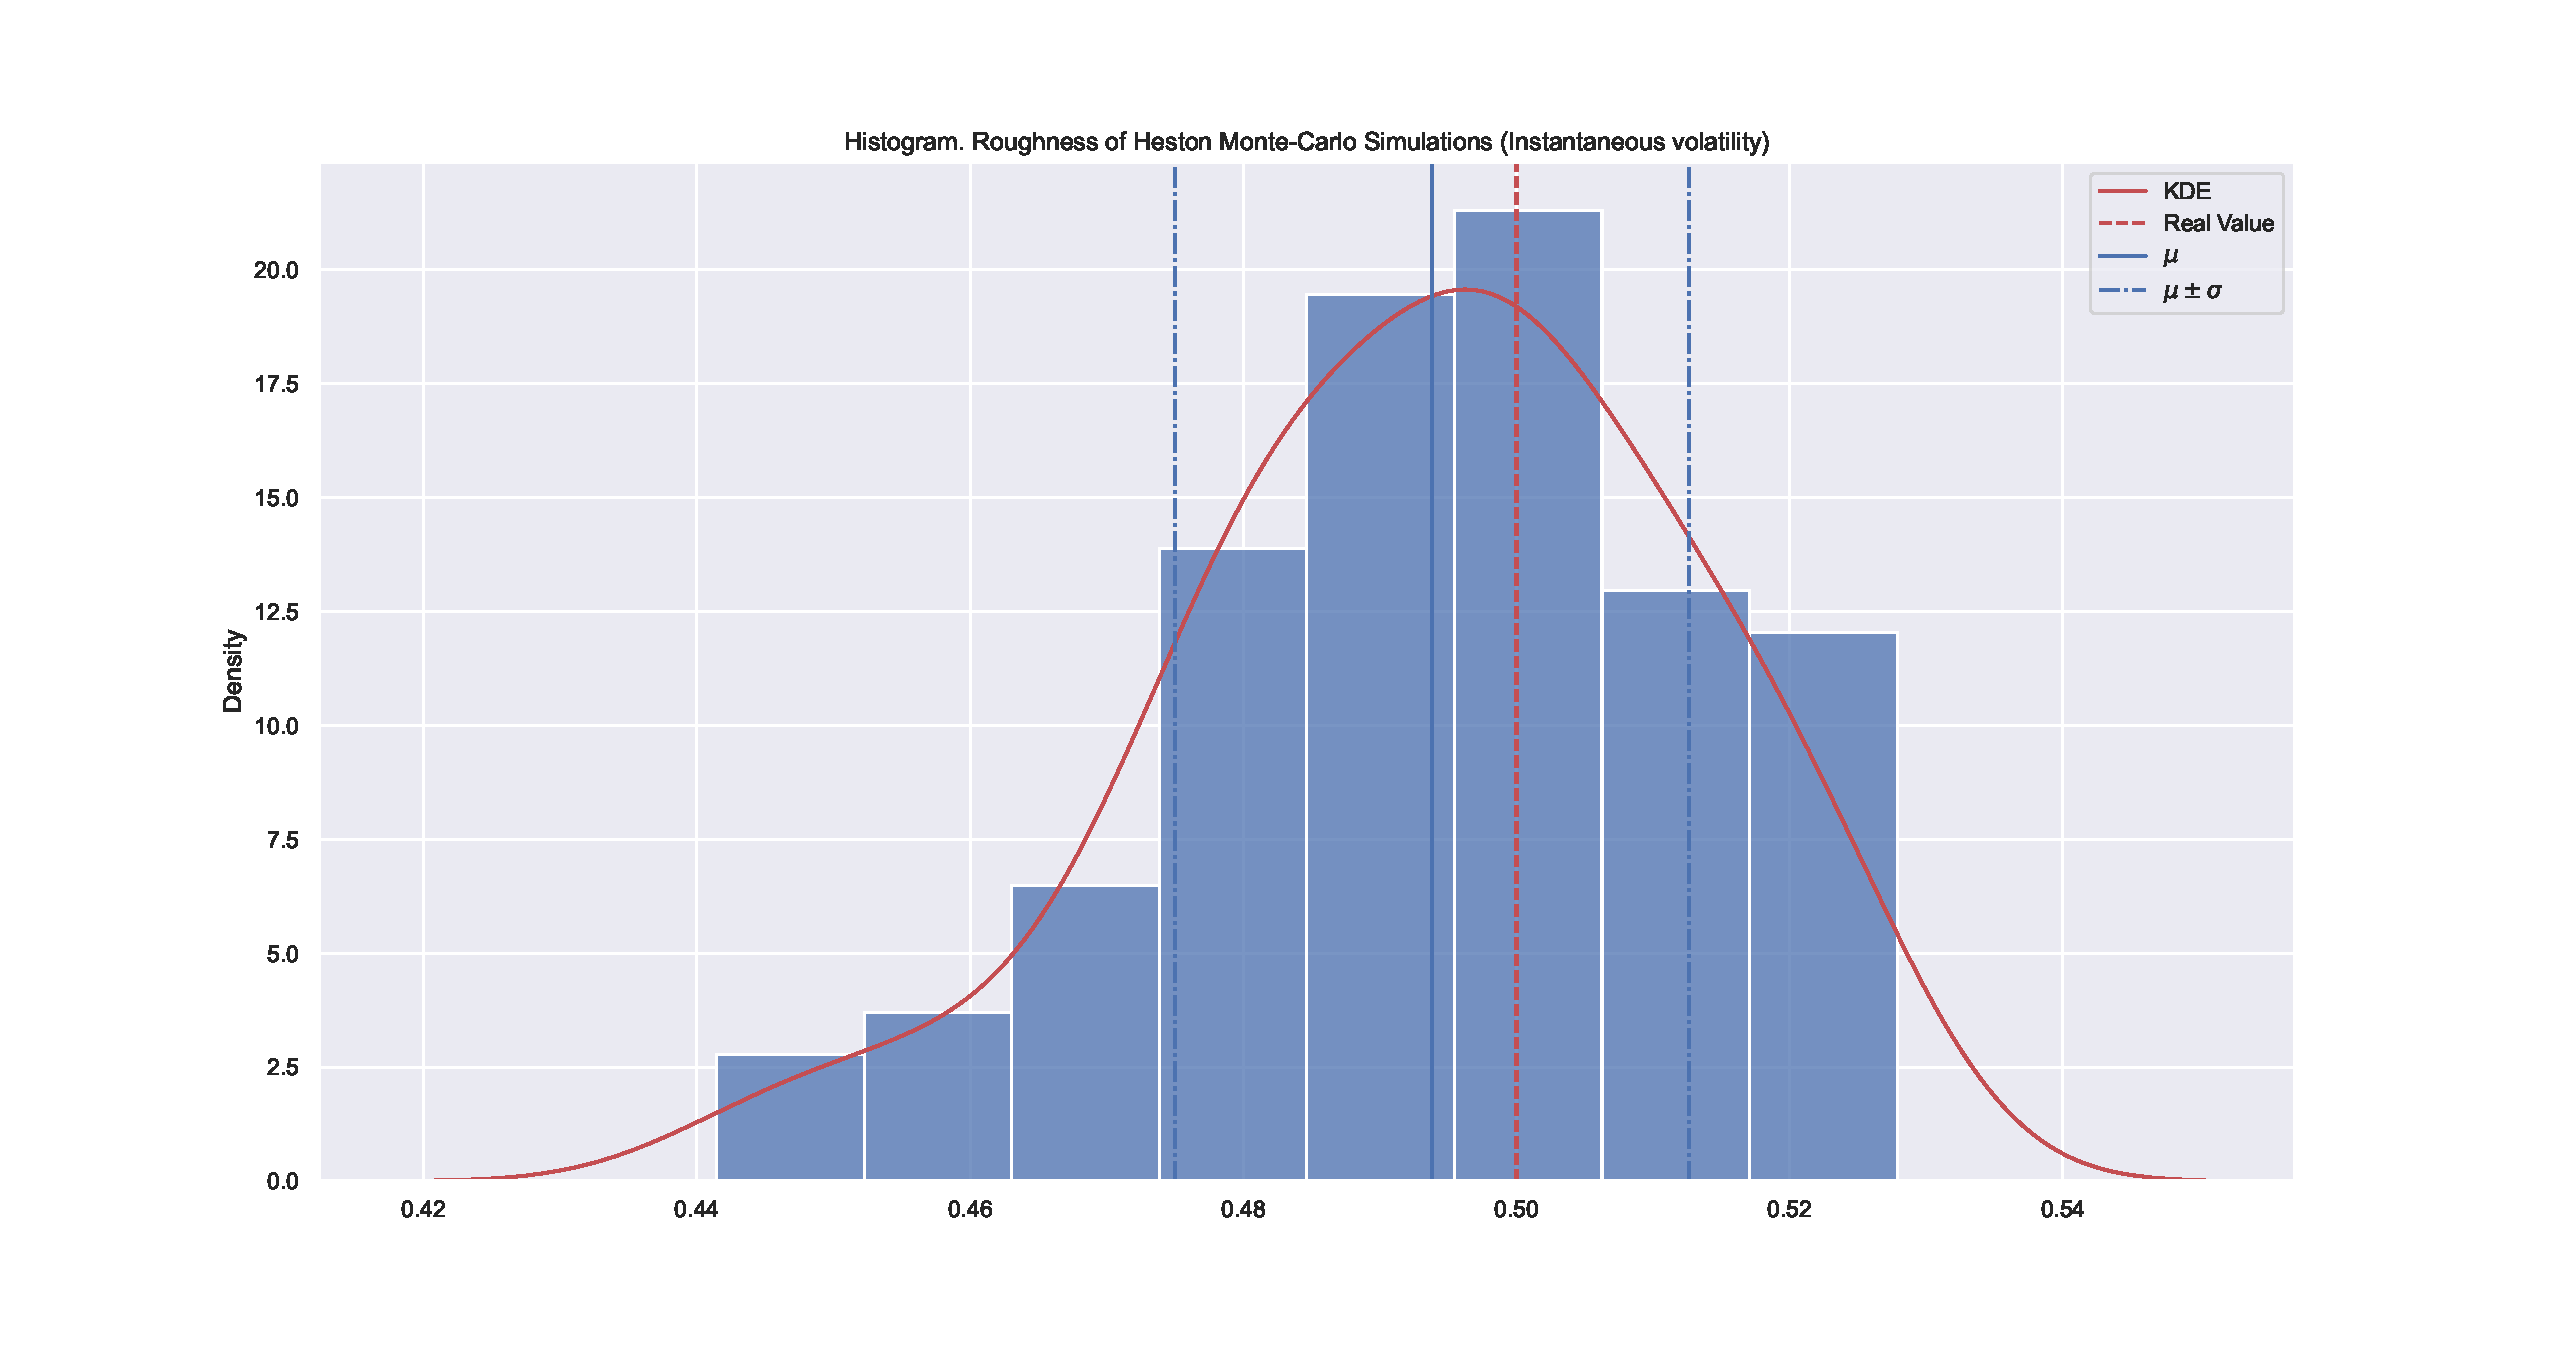
\includegraphics[width=\linewidth]{fig/Histogram. Roughness of Heston Monte-Carlo Simulations (Instantaneous volatility).pdf}
        \caption{Histogram for roughness of Heston SVM}
    \end{figure}
    \begin{figure}[htbp]
        \centering
        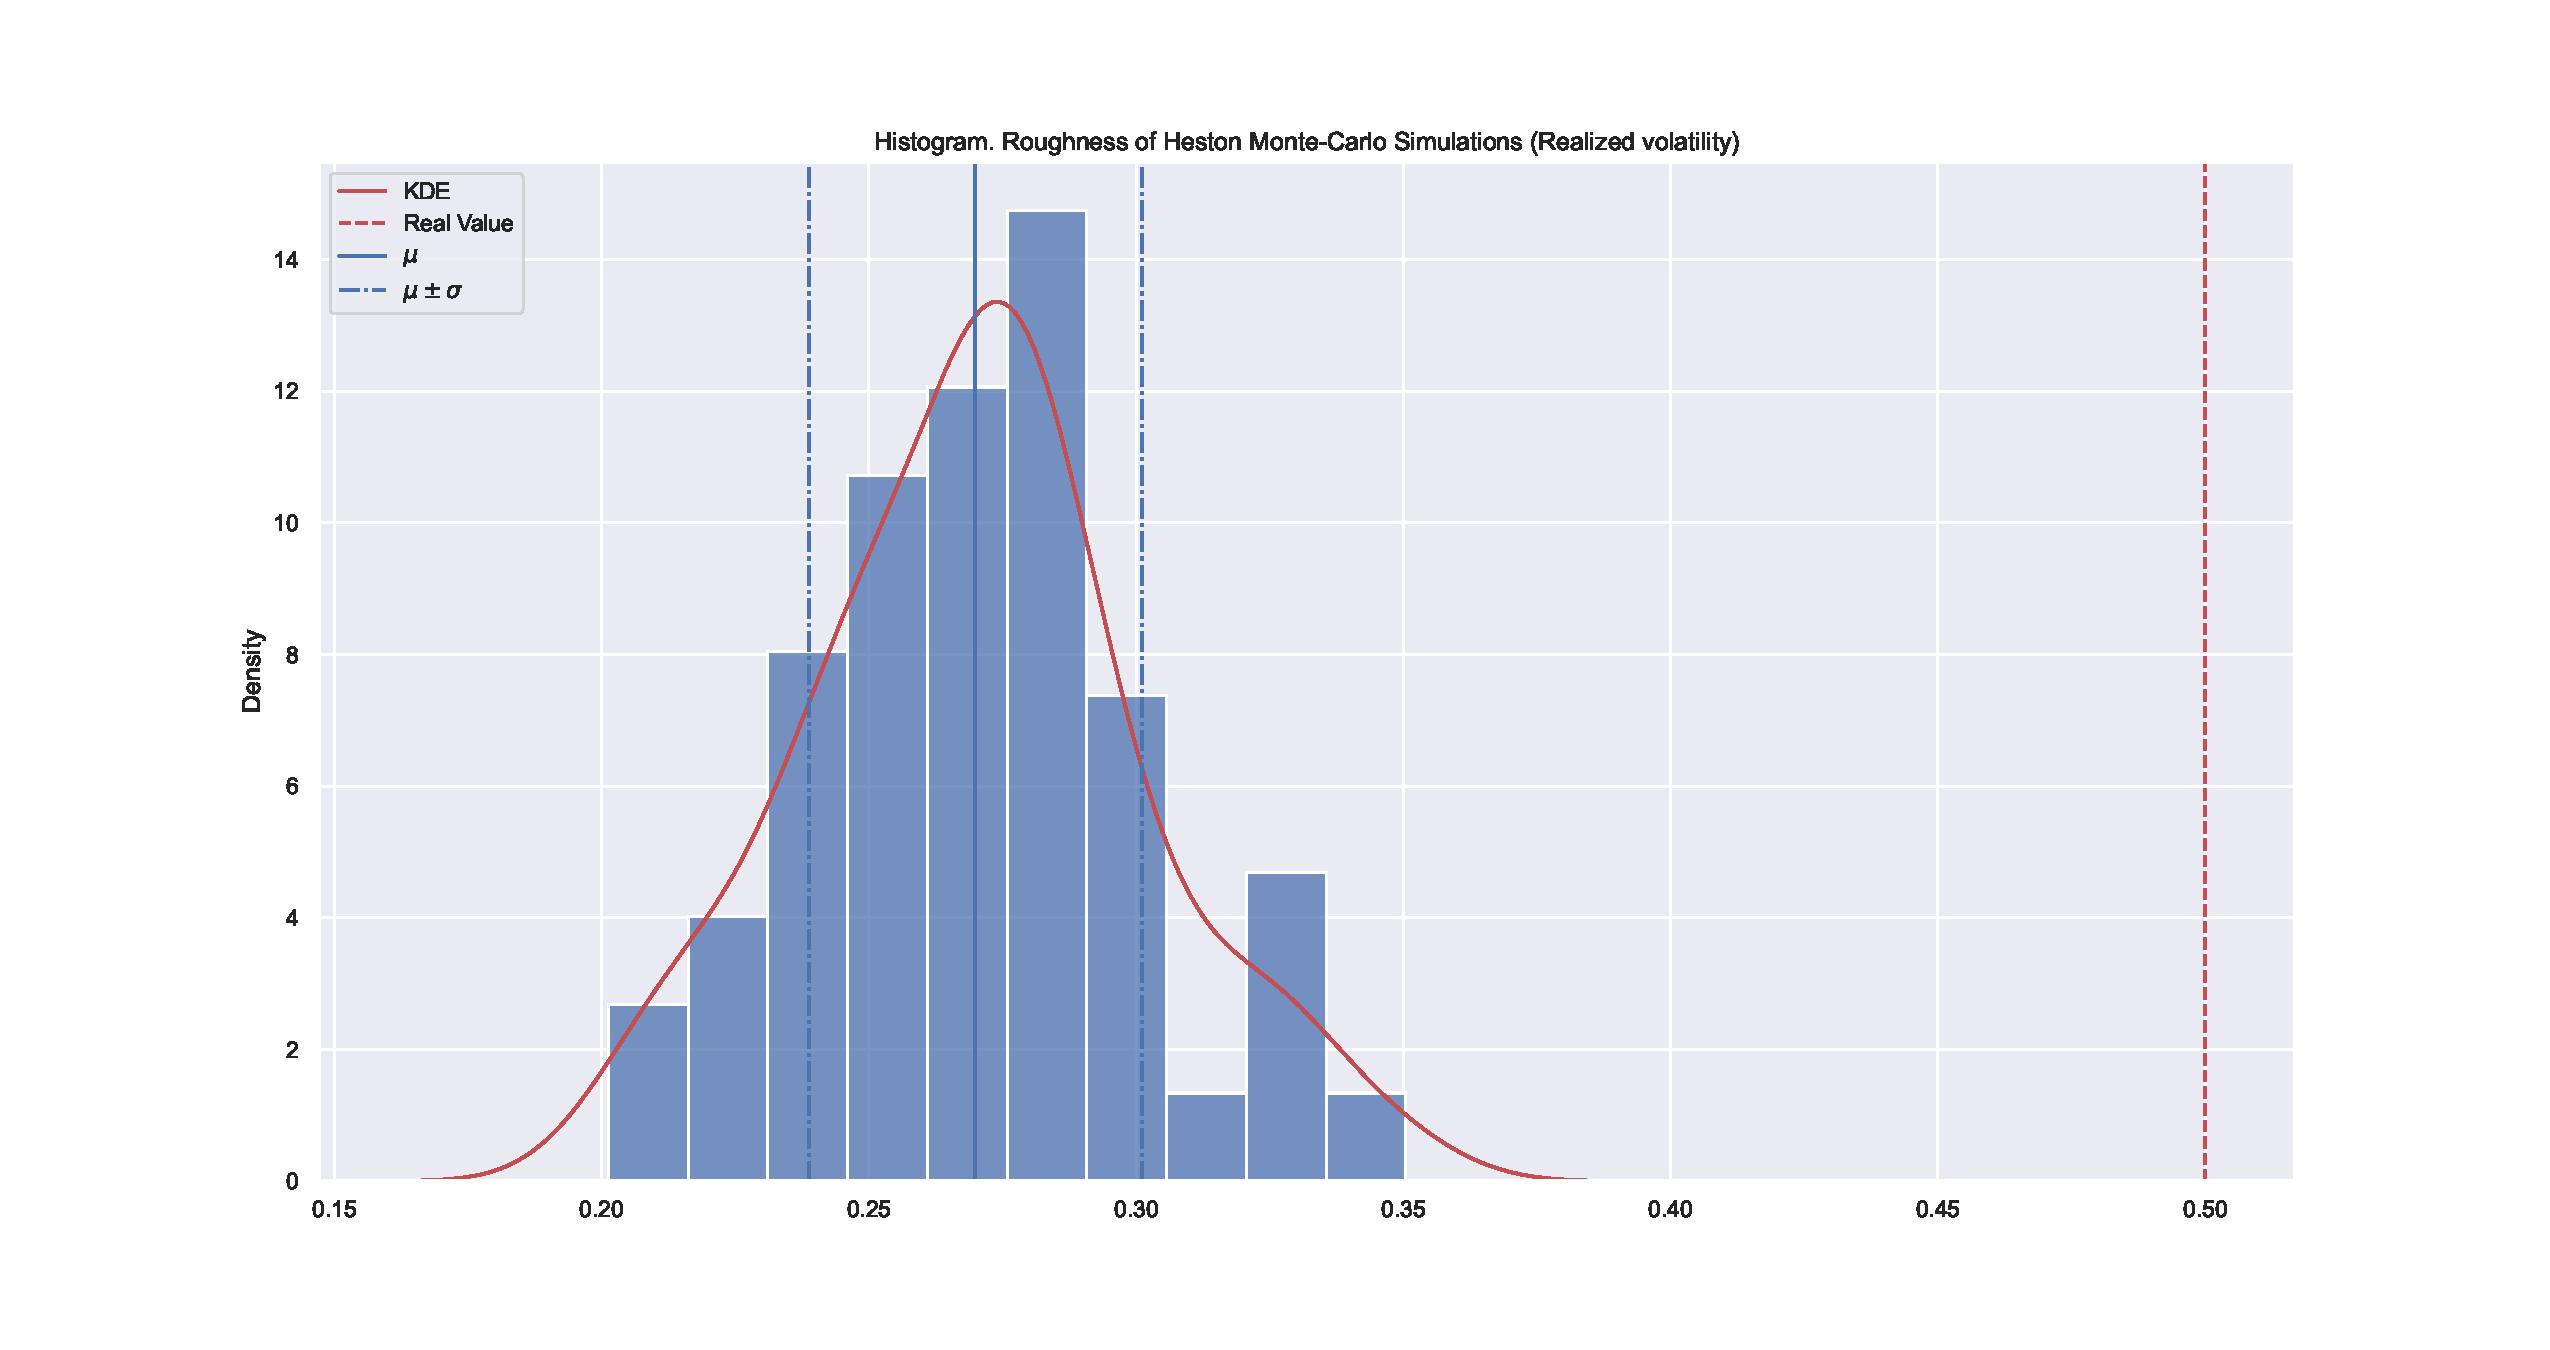
\includegraphics[width=\linewidth]{fig/Histogram. Roughness of Heston Monte-Carlo Simulations (Realized volatility).pdf}
        \caption{Histogram for roughness of Heston SVM}
    \end{figure}

\section{Roughness estimation of real-market data}

    Let us estimate the roughness of real-market data. 
    We are using the same Bloomberg data from Table \ref{table:hurst_est} (but without indexes).

    \begin{table}[h]
        \centering
        \begin{tabular}{|c|c|c|c|c|c|}
            \hline
            Ticker &  Roughness Index\\\hline
            \hline
            YNDX RX Equity & 0.372691\\\hline
            SBER RX Equity & 0.313109\\\hline
            VTBR RX Equity & 0.304677\\\hline
            MOEX RX Equity & 0.295378\\\hline
            LKOH RX Equity & 0.301795\\\hline
            GAZP RX Equity & 0.316125\\\hline
            FIVE RX Equity & 0.284704\\\hline
            \hline
            OGZD LI Equity & 2.968608\\\hline
            VTBR LI Equity & 0.306763\\\hline
            SBER LI Equity & 1.176616\\\hline
            LKOD LI Equity & 0.306061\\\hline
        \end{tabular}
        \caption{Roughness index estimation}
        \label{tab:roughness_index}
    \end{table}

    As we can see, modelless estimation of roughness differs from the Hurst parameter under RFSV (as Monte-Carlo simulations predicted).


    \addcontentsline{toc}{chapter}{Conclusion}\chapter*{Conclusion}

        \section{Conclusion}
    We got aquainted with the fractional stochastic volatility models framework and
    studied the statistical properties of RFSV. 
    We obtained roughness estimations for major Russian companies stocks and depositary 
    reciepts, and reproduced some effects described in \cite{GatheralRosenbaum2014}.

    \paragraph*{Reproduced hypotheses:}
    \begin{enumerate}
        \item The Hurst exponent of the considered assets has the order of $1e-1$ and is less than $\frac{1}{2}$.
        \item The volatility of the considered assets \textbf{does not} have a property of long memory under fractional stochastic 
                volatiltiy models.
        \item Visual analysis and normality tests for the log-increments of volatility shows that for 
              $\Delta \in [10, 25]$ the normality of log-inrements hypothesis holds.
        \item The smoothing effect holds for the estimations of $H$ and $\alpha$ (volatility of volatility under fOU). 
              But \textbf{only} for  VTBR LI Equity we got a negative slope of the smoothing effect. For other
              asset we got a nearly perfect linear fit and positive smoothing slopes.
    \end{enumerate}

    \addcontentsline{toc}{chapter}{Bibliography}\printbibliography

    \addcontentsline{toc}{chapter}{Appendix}\section{Appendix}
    
\end{document}